% /*@@
%   @file      ThornWriters.tex
%   @date      27 Jan 1999
%   @author    Gabrielle Allen, Tom Goodale, Gerd Lanfermann
%   @desc
%   Thorn writer's guide part of the Cactus User's Guide
%   @enddesc
%   @version $Header$
%   @history
%   @date     Tue Feb 12 14:33:25 CET 2002
%   @author   Jonathan Thornburg <jthorn@aei.mpg.de>
%   @desc     Revise section "Interpolation Operators" to cover the
%             new interpolation API (when we will have multiple APIs
%             coexisting, e.g. CCTK_InterpLocalUniform() and
%             CCTK_InterpLocalNonUniform())
%   @endhistory
% @@*/

\begin{cactuspart}{Thorn Writing}
\renewcommand{\thepage}{\Alph{part}\arabic{page}}
\label{part:ThornWriting}

\chapter{Application thorns}

%%%%%%%%%%%%%%%%%%%%%%%%%%%%%%%%%%%%%%%%%%%%%%%%%%%%%%%%%%%%%%%%%%%%%%%%%%%%%%%%
%%%%%%%%%%%%%%%%%%%%%%%%%%%%%%%%%%%%%%%%%%%%%%%%%%%%%%%%%%%%%%%%%%%%%%%%%%%%%%%%
%%%%%%%%%%%%%%%%%%%%%%%%%%%%%%%%%%%%%%%%%%%%%%%%%%%%%%%%%%%%%%%%%%%%%%%%%%%%%%%%

This chapter goes into the nitty-gritty of writing a thorn.
It introduces key concepts for thorns, then goes on to give
a brief outline of how to configure a thorn.
There is then some detail about concepts introduced by the configuration
step, followed by discussion of code which you must put into your files
in order to use Cactus functionality, and details of utility functions
you may use to gain extra functionality.

%%%%%%%%%%%%%%%%%%%%%%%%%%%%%%%%%%%%%%%%%%%%%%%%%%%%%%%%%%%%%%%%%%%%%%%
%%%%%%%%%%%%%%%%%%%%%%%%%%%%%%%%%%%%%%%%%%%%%%%%%%%%%%%%%%%%%%%%%%%%%%%

\section{Thorn Concepts}
\label{chap:thorn_concepts}

%%%%%%%%%%%%%%%%%%%%%%%%%%%%%%%%%%%%%%%%%%%%%%%%%%%%%%%%%%%%%%%%%%%%%%%

\subsection{Thorns}

A thorn is the basic working module within Cactus.  All user supplied
code goes into thorns, which are, by and large, independent of each other.
Thorns communicate with each other via calls to the flesh API, plus, more
rarely, custom APIs of other thorns.

The connection from a thorn to the flesh, or to other thorns, is specified in
configuration files which are parsed at compile time and used to generate
glue code which encapsulates the external appearance of a thorn.

Thorn names must be (case independently) unique, must start with a letter,
can only contain
letters, numbers or underscores, and must contain 27 characters or less.
In addition, a thorn cannot have the name \texttt{doc}, this is reserved
for arrangement documentation. Arrangement names which start with a
`\texttt{\#}', or finish with `\texttt{\~{}}' or `\texttt{.bak}' will be
ignored.

%%%%%%%%%%%%%%%%%%%%%%%%%%%%%%%%%%%%%%%%%%%%%%%%%%%%%%%%%%%%%%%%%%%%%%%

\subsection{Arrangements}
\label{sec:arrangements}

Thorns are grouped into \textit{arrangements}.  This is a logical grouping of
thorns which is purely for organisational purposes. For example,
you might wish to keep all your initial data thorns in one arrangement,
and all your evolution thorns in another arrangement, or you may want
to have separate arrangements for your developments, private and shared
thorns.

The arrangements live in the \texttt{arrangements} directory of the main
Cactus directory.  Arrangement names must be (case independently) unique,
must start with a letter,
and can only contain
letters, numbers or underscores. Arrangement names which start with a
`\texttt{\#}', or finish with `\texttt{\~{}}' or `\texttt{.bak}' will be
ignored.

Inside an arrangement directory there are directories for each thorn
belonging to the arrangement.

%%%%%%%%%%%%%%%%%%%%%%%%%%%%%%%%%%%%%%%%%%%%%%%%%%%%%%%%%%%%%%%%%%%%%%%

\subsection{Implementations}

\label{sec:implementations}

One of the key concepts for thorns is the concept of the \textit{implementation}.
Relationships among thorns are all based upon relationships among the
implementations they provide.
In principle, it should be possible to swap one thorn providing an
implementation with another thorn providing that implementation,
without affecting any other thorn.

An implementation defines a group of variables and parameters which
are used to implement some functionality.  For example, the thorn
\texttt{CactusPUGH/PUGH} provides the implementation \texttt{driver}.  This
implementation is responsible for providing memory for grid variables and
for communication.  Another thorn can also implement \texttt{driver},
and both thorns can be compiled in \emph{at the same time}.
At runtime, the user can decide which thorn providing \texttt{driver} is used.
No other thorn should be affected by this choice.

When a thorn decides it needs access to a variable or a parameter provided by
another thorn, it defines a relationship between itself and the other thorn's
\emph{implementation}, not explicitly with the other \emph{thorn}.
This allows the transparent replacement, at compile or runtime, of one
thorn with another thorn providing the same functionality as seen by
the other thorns.

%%%%%%%%%%%%%%%%%%%%%%%%%%%%%%%%%%%%%%%%%%%%%%%%%%%%%%%%%%%%%%%%%%%%%%%
%%%%%%%%%%%%%%%%%%%%%%%%%%%%%%%%%%%%%%%%%%%%%%%%%%%%%%%%%%%%%%%%%%%%%%%

\section{Anatomy of a Thorn}
\label{chap:thorn_anatomy}

%%%%%%%%%%%%%%%%%%%%%%%%%%%%%%%%%%%%%%%%%%%%%%%%%%%%%%%%%%%%%%%%%%%%%%%

\subsection{Thorns}

A thorn consists of a subdirectory of an arrangement containing four
administrative files:

\begin{Lentry}
\item[\texttt{interface.ccl}] the Cactus interface, which defines the grid
functions, variables, etc. See Appendix \ref{sec:Appendix.interface}.
\item[\texttt{param.ccl}] the parameters introduced by this thorn, and the
parameters needed from other thorns. See  Appendix 
\ref{sec:Appendix.param}.
\item[\texttt{schedule.ccl}] scheduling information for routines called by
the flesh. See Appendix  \ref{sec:Appendix.schedule}.
\item[\texttt{configuration.ccl}] configuration options for the thorn. See
 Appendix  \ref{sec:Appendix.configuration.ccl}.
\end{Lentry}

Thorns can also contain
\begin{itemize}
\item a subdirectory called \texttt{src}, which should hold source files
        and compilation instructions for the thorn
\item a subdirectory \texttt{src/include} for include files
\item a \texttt{README} containing a brief description of the thorn
\item a \texttt{doc} directory for documentation
\item a \texttt{par} directory for example parameter files
\item a \texttt{test} subdirectory may also be added, to hold the thorn's
    test suite. See Section \ref{sec:adding_test_suite} for details.
\end{itemize}

%%%%%%%%%%%%%%%%%%%%%%%%%%%%%%%%%%%%%%%%%%%%%%%%%%%%%%%%%%%%%%%%%%%%%%%

\subsection{Creating a Thorn}


To simplify the creation of a thorn, a \texttt{make} target {\tt
gmake newthorn} has been provided. When this is run:

\begin{enumerate}
\item{} You will be prompted for the name of the new thorn.
\item{} You will be prompted for the name of the arrangement in which you
would like to include your thorn. Either enter a new arrangement name or
pick one from the list of available arrangements that are shown.
\end{enumerate}

%%%%%%%%%%%%%%%%%%%%%%%%%%%%%%%%%%%%%%%%%%%%%%%%%%%%%%%%%%%%%%%%%%%%%%%

\subsection{Configuring your Thorn}

The interaction of a thorn with the flesh and other thorns is controlled
by certain configuration files.

These are:

\begin{Lentry}

\item [\texttt{interface.ccl}]
This defines the \textit{implementation} (Section~\ref{sec:implementations})
the thorn provides, and the variables the thorn needs, along with their
visibility to other implementations.

\item [\texttt{param.ccl}]
This defines the parameters that are used to control the thorn, along
with their visibility to other implementations.

\item [\texttt{schedule.ccl}]
This defines which functions are called from the thorn and when they are
called. It also handles memory and communication assignment for grid variables.

\item [\texttt{configuration.ccl}]
This file is optional for a thorn. If it exists, it contains extra
configuration options of this thorn.

\end{Lentry}

\subsubsection{General Syntax of CCL Files}

\textit{Cactus Configuration Language} (CCL) files are text files
used to define configuration information for a thorn. Their formal
syntax is described using Piraha, a parsing expression grammar engine
that supports multiple languages (see https://github.com/stevenrbrandt/piraha-peg
for a description of Piraha patterns and Grammar Files).

A Grammar File for each type of CCL file is provided in the src/piraha/pegs
directory of the Cactus source tree. These may be consulted for the precise
details of any given Cactus CCL file.

CCL files are
(mostly) case independent, and may contain comments introduced by the hash `\texttt{\#}'
character, which indicates that the rest of the line is a comment. If the last
non-blank character of a line in a CCL file is a backslash
`\texttt{$\backslash$}', the
following line is treated as a continuation of the current line.

\subsubsection{The \texttt{interface.ccl} File}
\label{subsec:interface_ccl}

The \texttt{interface.ccl} file is used to declare

\begin{itemize}
\item the implementation provided by the thorn
\item the variables provided by the thorn
\item the include files provided by the thorn
\item the functions provided by the thorn (in development)
\end{itemize}


The implementation is declared by a single line at the top of the file
\begin{alltt}
implements: <\var{name}>
\end{alltt}
Where \texttt{<\var{name}>} can be any combination of alphanumeric
characters and underscores, and is case independent.

There are three different access levels available for variables

\begin{Lentry}
\item[\texttt{Public}]
Can be `inherited' by other implementations (see below).
\item[\texttt{Protected}]
Can be shared with other implementations which declare themselves to
be friends of this one (see below).
\item[\texttt{Private}]
Can only be seen by this thorn.
\end{Lentry}

Corresponding to the first two access levels there are two relationship
statements that can be used to get variables (actually groups of variables,
see below) from other implementations.

\begin{Lentry}
\item [\texttt{Inherits: <\var{name}>}]
This gets all \texttt{Public} variables from implementation \texttt{<\var{name}>}, and all
variables that \texttt{<\var{name}>} has in turn inherited.
An implementation may inherit from any number of other implementations.
\item [\texttt{Friend: <\var{name}>}]
This gets all \texttt{Protected} variables from implementation \texttt{<\var{name}>}, but,
unlike \texttt{inherits}, it is symmetric and also defines a transitive relation by
pushing its own implementation's \texttt{Protected} variables onto implementation
\var{name}.  This keyword is used to define a group of implementations which
all end up with the same \texttt{Protected} variables.
\end{Lentry}

So, for example, an \texttt{interface.ccl} starting
\begin{alltt}
implements: wavetoy
inherits:   grid
friend:     wave_extract
\end{alltt}
declares that the thorn provides an implementation called \texttt{wavetoy}, gets
all the \texttt{public} variables declared by an implementation called \texttt{grid},
and shares all \texttt{protected} variables with \texttt{wave\_extract} and its
friends.

Cactus variables, described in Chapter~\ref{chap:cactus_variables}, are placed
in groups with homogeneous attributes, where
the attributes describe properties such as the data type, group type,
dimension, ghostsize, number of timelevels, and
distribution.

For example, a group, called \texttt{realfields} of 5 real grid
functions (\texttt{phi}, \texttt{a},
\texttt{b}, \texttt{c}, \texttt{d}), on a 3D grid, would be defined by
\begin{verbatim}
CCTK_REAL realfields type=GF TimeLevels=3 Dim=3
{
  phi
  a,b,c,d
} "Example grid functions"
\end{verbatim}
or, for a group called \texttt{intfields} consisting of just one
distributed 2D array of integers,
\begin{verbatim}
CCTK_INT intfields type=ARRAY size=xsize,ysize ghostsize=gxsize,gysize dim=2
{
 anarray
} "My 2D arrays"
\end{verbatim}
where \texttt{xsize}, \texttt{ysize}, \texttt{gxsize}, \texttt{gysize} are all
parameters defined in the thorn's \texttt{param.ccl}.


By default, all groups are \texttt{private}, to change this, an access
specification of the form \texttt{public:} or \texttt{protected:} (or
\texttt{private:} to change it back) may be placed on a line by itself.  This
changes the access level for any group defined in the file from that point on.

All variables seen by any one thorn must have distinct names.

\subsubsection{The \texttt{param.ccl} File}
\label{subsec:param_ccl}

Users control the operation of thorns via parameters given in a file
at runtime.  The \texttt{param.ccl} file
is used to specify the parameters used to control an individual thorn, and
to specify the values these parameters are allowed to take.  When the code
is run, it reads a parameter file and sets the parameters if they fall
within the allowed values. If a parameter is not assigned in a parameter
file, it is given its default value.

There are three access levels available for parameters:

\begin{Lentry}
\item [\texttt{Global}]
These parameters are seen by all thorns.
\item [\texttt{Restricted}]
These parameters may be used by other implementations if they so desire.
\item [\texttt{Private}]
These are only seen by this thorn.
\end {Lentry}

A parameter specification consists of:
\begin{itemize}

\item The parameter type (each may have an optional {\t CCTK\_} in front)
\begin{Lentry}
\item [\texttt{REAL}]
\item [\texttt{INT}]
\item [\texttt{KEYWORD}]
A distinct string with only a few known allowed values.
\item [\texttt{STRING}]
An arbitrary string, which must conform to a given regular expression.
\item [\texttt{BOOLEAN}]
A boolean type which can take values {\t 1}, {\t t}, {\t true}, {\t yes} or
{\t 0}, {\t f}, {\t false}, {\t no}.
\end{Lentry}

\item The parameter name

\item An optional size (in square brackets)--if this is present, the
  parameter is a ``parameter array'', i.e.\ it will actually be an array
  of parameters, each of which has the same properties, but a different
  value.  Such arrays appear as normal arrays in C or Fortran, 0-based
  in C, and 1-based in Fortran.  In the parameter file the value of
  each element is specified with square brackets and is 0-based.  The
  size must be an integer.

\item A description of the parameter

\item An allowed value block--this consists of a brace-delimited
block of lines\footnote{The beginning brace (\texttt{\{}) must sit on a line by
itself; the ending brace (\texttt{\}}) must be preceded by a carriage return.}
describing the allowed values of the parameter.  Each range may have a
description associated with it by placing a \texttt{::} on the line, and putting
the description afterwards.

\item The default value--this must be one of the allowed values.

\end{itemize}

For the numeric types \texttt{INT} and \texttt{REAL}, a range consists
of a string of the
form lower-bound:upper-bound:step, where a missing number or an asterisk
`\texttt{*}' denotes anything (i.e.\ infinite bounds or an infinitesimal step).

For example,
\begin{verbatim}
REAL Coeff "Important coefficient"
{
0:3.14 :: "Range has to be from zero to Pi, default is zero"
} 0.0

#No need to define a range for BOOLEAN
BOOLEAN nice "Nice weather?"
{
}"yes"

# A example for a set of keywords and its default (which has to be
# defined in the body)
KEYWORD confused "Are we getting confused?"
{
  "yes"    :: "absolutely positively"
  "perhaps" :: "we are not sure"
  "never"   :: "never"
} "never"

REAL Length[2] "Length in each direction"
{
0:* :: "Range has to be from zero to infinity, default is one"
} 1.0

\end{verbatim}
defines a \texttt{REAL} parameter, a \texttt{BOOLEAN} parameter, a \texttt{KEYWORD},
and an array of \texttt{REAL} parameters.

By default, all parameters are \texttt{private}; to change this, an access
specification of the form \texttt{global:} or \texttt{restricted:} (or
\texttt{private:} to change it back) may be placed on a line by itself.  This
changes the access level for any parameter defined in the file from that point on.

To access \texttt{restricted} parameters from another implementation, a line
containing \texttt{shares: <\var{name}>} declares that all parameters mentioned in
the file, from now until the next access specification, originate in
implementation \texttt{<\var{name}>}. (Note that only one implementation can be
specified on each \texttt{shares:} line.)  Each of these parameters must be qualified by the initial token \texttt{USES} or \texttt{EXTENDS}, where
\begin{Lentry}
\item[\texttt{USES}] indicates that the parameters range remains unchanged.
\item[\texttt{EXTENDS}] indicates that the parameters range is going to be extended.
\end{Lentry}

In contrast to parameter declarations in other access blocks, the default
value must be omitted---it is impossible to set the default value of any
parameter not originating in this thorn.
For example, the following block adds possible values to the keyword
\texttt{initial\_data} originally defined in the implementation \texttt{einstein},
and uses the \texttt{REAL} parameter \texttt{speed}.

\begin{verbatim}
shares:einstein

EXTENDS KEYWORD initial_data
{
  "bl_bh"         :: "Brill Lindquist black holes"
  "misner_bh"     :: "Misner black holes"
  "schwarzschild" :: "One Schwarzschild black hole"
}

USES CCTK_REAL speed

\end{verbatim}

Note that you must compile at least one thorn which implements \texttt{einstein}.


%%%%%%%%%%%%%%%%%%%%%%%%%%%%%%%%%%%%%%%%%%%%%%%%%%%%%%%%%%%%%%%%%%%%%%%%%%%
%%%%%%%%%%%%%%%%%%%%%%%%%%%%%%%%%%%%%%%%%%%%%%%%%%%%%%%%%%%%%%%%%%%%%%%%%%%

\subsubsection{The \texttt{schedule.ccl} File}
\label{subsec:schedule_ccl}
By default, no routine of a thorn will be run.  The \texttt{schedule.ccl}
file defines those that should be run, and when and under which
conditions they should be run.

The specification of routine scheduling is via a schedule block which
consists of lines of the form

\begin{alltt}
schedule <\var{name}> at <\var{time bin}> [\var{other options}]
\{
  LANG:     <FORTRAN|C>
  OPTIONS:     [\var{list of options}]
  TAGS:        [\var{list of keyword=value definitions}]
  STORAGE:     [\var{group list with timelevels}]
  READS:       [\var{variable or group list with region specification}]
  WRITES:      [\var{variable or group list with region specification}]
  TRIGGERS:    [\var{group list}]
  SYNC:        [\var{group list}]
\} "\var{A description}"
\end{alltt}
where \texttt{<\var{name}>} is the name of the routine, and
\texttt{<\var{time bin}>} is the name of a schedule bin (the \texttt{CCTK\_}
prefix is optional). A list of the most useful schedule bins for application
thorns is given here, a complete and more descriptive list is provided in
Appendix~\ref{sec:Appendix.schedule_bins}:

\begin{Lentry}

\item [\texttt{CCTK\_STARTUP}]
For routines, run before the grid hierarchy is set up, for example, function
registration.

\item [\texttt{CCTK\_PARAMCHECK}]
For routines that check parameter combinations, routines registered here
only have access to the grid size and the parameters.

\item [\texttt{CCTK\_BASEGRID}]
Responsible for setting up coordinates, etc.

\item [\texttt{CCTK\_INITIAL}]
For generating initial data.

\item [\texttt{CCTK\_POSTINITIAL}]
Tasks which must be applied after initial data is created.

\item [\texttt{CCTK\_PRESTEP}]
Stuff done before the evolution step.

\item [\texttt{CCTK\_EVOL}]
The evolution step.

\item [\texttt{CCTK\_POSTSTEP}]
Stuff done after the evolution step.

\item [\texttt{CCTK\_ANALYSIS}]
For analysing data.

\end{Lentry}

The \var{other options} allow finer-grained control of the scheduling.  It is
possible to state that the routine must run \texttt{BEFORE} or \texttt{AFTER}
another routine or set of routines.
It is also possible to schedule the routine under an
alias name by using \texttt{AS <\var{alias\_name}>}.

\begin{Lentry}

\item[\texttt{LANG}]
The \texttt{LANG} keyword specifies the linkage of the scheduled routine
which determines how to call it from the scheduler.
C and Fortran linkage are possible here. C++ routines should be defined as
\texttt{extern "C"} and registered as \texttt{LANG: C}.

\item[\texttt{OPTIONS}] Schedule options are used for mesh refinement
  and multi-block simulations, and they determine ``where'' a routine
  executes. Often used schedule options are \texttt{local} (also the
  default, may be omitted), \texttt{level}, or \texttt{global}.
  Routines scheduled in \emph{local mode} can access individual grid
  points, routines scheduled in \emph{level mode} are used e.g.\ to
  select boundary conditions, and routines schedule in \emph{global
    mode} are e.g.\ used to calculate reductions (norms).

\item[\texttt{TAGS}] Schedule tags, e.g.\ \texttt{Device=1} to specify
  that a routine executes on an OpenCL or CUDA device instead of on
  the host.

\item[\texttt{STORAGE}] The \texttt{STORAGE} keyword specifies any groups for
which memory should be allocated for the duration of the routine.  The
storage status reverts to its previous status after the routine
returns. The format of the \texttt{STORAGE} statement includes specifying
the number of timelevels of each group for which storage should be activated.

\texttt{STORAGE: <\var{group1}>[\var{timelevels1}],
<\var{group2}>[\var{timelevels2}]}

 This number can range from one to the maximum number of timelevels for the group, as specified in the group definition in its \texttt{interface.ccl} file. If this maximum number is one, the timelevel specification can be omitted from the
\texttt{STORAGE} statement.
Alternatively \var{timelevels} can be the name of a parameter accessible
to the thorn. The parameter name is the same as used in C routines of the
thorn, fully qualified parameter names of the form
\texttt{\var{thorn}::\var{parameter}} are not allowed. In this case 0 (zero)
\var{timelevels} can be requested, which is equivalent to the {\tt STORAGE}
statement being absent.

\item[\texttt{READS/WRITES}] \texttt{READS/WRITES} are used to
  declare which grid variables are read/written by the routine. This information is
  used e.g.\ to determine which variables need to be synchronized, copied between host
  and device for OpenCL or CUDA kernel, or poisoned as part of error checking. 

  READS/WRITE directives can be applied to either a variable or a group of
  variables and may also contain a region specification. The region specification can
  be EVERYWHERE, INTERIOR, or BOUNDARY. If a function needs to read a given grid function
  everywhere and only the interior is valid (i.e. has been written to), then a synchronization
  is required and will happen automatically if enabled with the Cactus parameter \texttt{presync\_mode}.

  When grid functions are updated in this way, not only ghost zones, but boundary zones
  will be updated by the drier.  Use either the function
  \texttt{Driver\_SelectGroupForBC} or \texttt{Driver\_SelectVarForBC} to tell the driver how it should update a group or variable. The
  arguments to both functions are the same as those found in the
  Boundary thorn, but with the prefix \texttt{Boundary\_} instead of
  \texttt{Driver\_}:

\begin{verbatim}
Driver_SelectGroupForBC(CCTK_ARGUMENTS,
                        CCTK_INT faces,
                        CCTK_INT width,
                        CCTK_INT table_handle,
                        CCTK_STRING group_name,
                        CCTK_STRING bc_name)

Driver_SelectVarForBC(CCTK_ARGUMENTS,
                      CCTK_INT faces,
                      CCTK_INT width,
                      CCTK_INT table_handle,
                      CCTK_STRING var_name,
                      CCTK_STRING bc_name)
\end{verbatim}

Note that the above two functions, unlike their similarly named components in the Boundary thorn, only need to be called once. The information they provide will then be used each time the driver synchronizes the named grid function or group.

It is possible, however, that the thorn you are creating does not know the correct READS/WRITES information at compile time. I/O thorns, for
example, do not know which grid functions they will access until run time. Likewise, the Method of Lines thorn does not know which grid functions it is operating on until run time.

For situations like these, we have the following functions which can be used to check READS/WRITES data and perform synchronization at run time:
\texttt{Driver\_RequireValidData}, \texttt{Driver\_NotifyDataModified}, \texttt{Driver\_GetValidRegion}, and \texttt{Driver\_SetValidRegion}. For details on these functions, please consult the Reference Manual.

\item[\texttt{TRIGGERS}] \texttt{TRIGGERS} is used when the routine is
registered at \texttt{ANALYSIS}.  This is a special time bin; a routine
registered here will only be called if one of the variables from a
group in \texttt{TRIGGERS} is due for output.  (A routine without {\tt
TRIGGERS} declaration will always be called.)

\item[\texttt{SYNC}]
The keyword \texttt{SYNC} specifies groups of variables which should be
synchronised (that is, their ghostzones should be exchanged between
processors) on exit from the routine. Specifying synchronisation of
grid variables in \texttt{schedule.ccl} is an alternative to calling the
functions \texttt{CCTK\_SyncGroup()} or \texttt{CCTK\_SyncGroupsI()}
(see the Reference Manual) from inside a routine. Using the \texttt{SYNC}
keyword in the \texttt{schedule.ccl} is the preferred method, since it
provides the flesh with more information about the behaviour of your code.

As an alternative to this mechanism, synchornization can happen automatically
as variables are read/written.


\end{Lentry}

Besides schedule blocks, it's possible to embed C style \texttt{if/else}
statements in the \texttt{schedule.ccl} file.  These can be used to
schedule things based upon the value of a parameter.

\vskip .5cm
{\bf Example I:}

If the parameter \texttt{evolve\_hydro} is positively set, the Fortran
routine \texttt{hydro\_predictor} is scheduled to run in the \textit{evolution}
loop, after the routine \texttt{metric\_predictor} and before
\texttt{metric\_corrector}. The routine names \texttt{metric\_predictor} and
\texttt{metric\_corrector}, may either be real routine names from the same
or a different thorn, or they may be \texttt{aliased} routine names (see the
next example).

Before entry to \texttt{hydro\_predictor},
storage will be allocated for one timelevel for the group of grid
variables \texttt{hydro\_variables} on exit from the routine this storage
will be deallocated and the contents of the variables will be lost.
\begin{verbatim}
if(CCTK_Equals(evolve_hydro,"yes"))
{
  SCHEDULE hydro_predictor AT evol AFTER metric_predictor BEFORE metric_corrector
  {
    LANG:     FORTRAN
    STORAGE:  hydro_variables[1]
  } "Do a predictor step on the hydro variables"
}
\end{verbatim}

If the parameter \texttt{evolve\_hydro} is set negatively, the {\tt
hydro\_predictor} routine will not be called by the scheduler. Note
that if the \texttt{evolve\_hydro} parameter is \texttt{STEERABLE}, it can be
dynamically scheduled and de-scheduled during a run if a steering
interface is available.

\vskip .5cm
{\bf Example II:}

The thorns \texttt{WaveToy77} and \texttt{WaveToyC}, each provide a
routine to evolve the 3D wave equation: \texttt{WaveToyF77\_Evolution} and
\texttt{WaveToyC\_Evolution}. The routine names have to be different, so
that both thorns can be compiled at the same time, their functionality
is identical though. Either one of them can then be activated at run
time  in the parameter file via \texttt{ActiveThorns}.

Since each evolution routine provides the same
functionality, it makes sense to schedule them under the common alias {\tt
WaveToy\_Evolution} to allow relative scheduling ({\tt
BEFORE/AFTER}) independent of the actual routine name (which may
change depending on the activation in the parameter file).

In both cases, the group of variables \texttt{scalarfield} are synchronised
across processes when the routine is exited.
\begin{verbatim}
schedule WaveToyF77_Evolution AS WaveToy_Evolution AT evol
{
  LANG: Fortran
  STORAGE: scalartmps
  SYNC: scalarfield
} "Evolution of 3D wave equation"

schedule WaveToyC_Evolution AS WaveToy_Evolution AT evol
{
  LANG: C
  STORAGE: scalartmps
  SYNC: scalarfield
} "Evolution of 3D wave equation"
\end{verbatim}
The thorn \texttt{IDScalarWave} schedules the routine \texttt{WaveBinary}
after the alias \texttt{WaveToy\_Evolution}. It is scheduled independently of
the C or Fortran routine name.
\begin{verbatim}
schedule WaveBinary AT evol AFTER WaveToy_Evolution
{
  STORAGE: wavetoy::scalarevolve
  LANG:    Fortran
} "Provide binary source during evolution"
\end{verbatim}

\paragraph{Storage Outside of Schedule Blocks}
The keyword \texttt{STORAGE} can also be used outside of the schedule
blocks to indicate that storage for these groups should be switched on
at the start of the run. Note that the storage is only allocated in
this way at the start; a thorn could explicitly switch the storage off
(although this is not recommended practise). As for the \texttt{STORAGE}
statement in schedule blocks, each group must also specify how many
timelevels to activate storage for.

%%%%%%%%%%%%%%%%%%%%%%%%%%%%%%%%%%%%%%%%%%%%%%%%%%%%%%%%%%%%%%%%%%%%%%%%%%%
%%%%%%%%%%%%%%%%%%%%%%%%%%%%%%%%%%%%%%%%%%%%%%%%%%%%%%%%%%%%%%%%%%%%%%%%%%%

\subsubsection{The \texttt{configuration.ccl}}
\label{subsec:configuration_ccl}

The \texttt{configuration.ccl} file is optional.  It can be used for two
purposes: to detect certain features of the host system, such as the
presence or absence of libraries, variable types, etc, or the
location of libraries; or to provide access to certain functions too
complex or otherwise not suitable for function aliasing.

The basic concept here is that a thorn can either provide or use a
{\bf capability}.  A thorn providing a capability can specify a script
which is run by the CST to detect features and write any configuration
files;  the script may output lines to its standard output to inform
the CST of features to: add to the header files included by thorns
using this capability; add to the make files used to build thorns
using this capability; or add to the main Cactus link line.  The script
may also indicate that this capability is not present by returning a
non-zero exit code---e.g. if the thorn is providing access to an
external library, it should return an error if the library is not
installed on the system.

A thorn may either require a capability to be present, in which case
it is an error if there is no thorn providing that capability in the
configuration's \texttt{ThornList}, or it may optionally use a capability, in
which case a macro is defined in the thorn's header file if a thorn
providing the capability is present.

A configuration.ccl file has the form:

\begin{alltt}
PROVIDES <\var{My_Capability}>
\{
  SCRIPT <\var{My_ConfigScript}>
  LANG <\var{My_Language}>
\}

REQUIRES  <\var{Another_Capability}>

OPTIONAL <\var{Yet_Another_Capability}>
\{
%  DEFINE <\var{macro}>
\}

\end{alltt}

which states that this thorn provides the capability
\verb|My_Capability|, and a script \verb|MyConfigScript| should be run
to detect features of this capability; the script is in language
\verb|My_Language|---the CST will use the appropriate environment or
interpreter to invoke the script.

% The example requires a thorn providing \verb|Another_Capability| to be
% in the \texttt{ThornList}, and, if a thorn providing
% \verb|Yet_Another_Capability| is in the \texttt{ThornList}, the preprocessor
% macro \verb|macro| will be defined, and set to 1.
% 
% As an example, a thorn A may be able to use PVM for parallelism if it is
% present, but can still work in the absence of it.  There could be a
% thorn providing PVM, and thorn A would then have
% 
% \begin{alltt}
% OPTIONAL PVM
% \{
%   DEFINE HAVE_PVM
% \}
% 
% \end{alltt}
% 
% The code in thorn A could then have
% 
% \begin{alltt}
% 
% #ifdef HAVE_PVM
%   do something
% #else
%   do something else
% #endif
% 
% \end{alltt}
% 
% to pick the appropriate mode.

The syntax of the output of the configure script is described in
Appendix \ref{sec:Appendix.configuration.ccl.configscript}.


%%%%%%%%%%%%%%%%%%%%%%%%%%%%%%%%%%%%%%%%%%%%%%%%%%%%%%%%%%%%%%%%%%%%%%%
%%%%%%%%%%%%%%%%%%%%%%%%%%%%%%%%%%%%%%%%%%%%%%%%%%%%%%%%%%%%%%%%%%%%%%%

\subsection{Naming Conventions for Source Files}
\label{nacofosofi}

The make system uses file extensions to designate coding language,
as well as other properties of the code in the file.

The following extensions are understood:

\begin{center}
\begin{tabular}{|l|c|c|c|}
\hline
Extension            & Language               &  Preprocess \\
\hline
{\t .c}              & C                      & yes \\
{\t .cc} or {\t .C}  & C++                    & yes \\
{\t .cl}             & OpenCL                 & yes \\
{\t .cu}             & CUDA                   & yes \\
{\t .F} or {\t .F77} & Fortran (fixed-format) & yes \\
{\t .f} or {\t .f77} & Fortran (fixed-format) & no  \\
{\t .F90}            & Fortran (free-format)  & yes \\
{\t .f90}            & Fortran (free-format)  & no  \\
\hline
\end{tabular}
\end{center}

In order to use Cactus \texttt{\#include} directives in a file, it must be
preprocessed.

A complete description of Fortran fixed and free format can be found in any
textbook on Fortran.  The most obvious differences are that in fixed
format, code must begin after the 5th column and line continuations are
indicated by a character in column 5, while in free format, lines can begin
anywhere, and line continuations are indicated by an ampersand at the end of
the line to be continued.  Also note that statement labels are handled
very differently.

The following restrictions apply to file names:
\begin{itemize}
\item For portability across all operating systems, the base names
        for any particular extension should not depend on the operating
        system being case sensitive (e.g.\ having \texttt{MyFile.c} and
        \texttt{MYFILE.f} is allright, but \texttt{MyFile.c} and
	\texttt{MYFILE.c} could cause problems).
\item Currently, all source files within a thorn must have distinct names,
regardless of whether they are placed in different subdirectories.  We hope
to relax this in future.  Different thorns may have files with the same names,
however.
\end{itemize}

%%%%%%%%%%%%%%%%%%%%%%%%%%%%%%%%%%%%%%%%%%%%%%%%%%%%%%%%%%%%%%%%%%%%%%%

\subsection{Adding Source Files}

By default, the CCTK looks in the \texttt{src} directory of the thorn for source
files.

There are two ways in which to specify the sources.  The easiest is to use the
\texttt{make.code.defn} based method in which the CCTK does all the work, but you
may instead put a \texttt{Makefile} in the \texttt{src} directory and do everything
yourself.

\subsubsection{\texttt{make.code.defn} based thorn building}
\label{sec:mabathbu}

This is the standard way to compile your thorn's source files.
The Cactus make system looks for a file called \texttt{make.code.defn} in that
directory (if there is no file called \texttt{Makefile} in the \texttt{src} directory).  At its simplest, this file contains two lines

\begin{itemize}
\item \texttt{SRCS = <\var{list of all source files in this directory}>}

\item \texttt{SUBDIRS = <\var{list of all subdirectories, including
subdirectories of subdirectories}>}

\end{itemize}

Each subdirectory listed should then have a \texttt{make.code.defn} file
containing just a \texttt{SRCS = } line, a \texttt{SUBDIRS = } line will
be ignored.

In addition, each directory can have a \texttt{make.code.deps} file, which,
for files in that directory, can contain additional make rules and dependencies
for files in that directory.  See the GNU Make documentation for complete details of the
syntax.

\subsubsection{\texttt{Makefile} based thorn building}

This method gives you the ultimate responsibility.
The only requirement is that
a library called \texttt{\$NAME} be created by the \texttt{Makefile}.

The makefile is passed the following variables
\begin{Lentry}

\item [\texttt{\$(CCTK\_HOME)}]  the main Cactus directory

\item [\texttt{\$(TOP)}] the configuration directory

\item [\texttt{\$(SRCDIR)}] the directory in which the source files can be found

\item [\texttt{\$(CONFIG)}]  the directory containing the configuration files

\item [\texttt{\$(THORN)}]   the thorn name

\item [\texttt{\$(SCRATCH\_BUILD)}]  the scratch directory where Fortran module
files should end up if they need to be seen by other thorns.

\item [\texttt{\$(NAME)}] the name of the library to be built

\end{Lentry}

and has a working directory of
\texttt{<\var{config}>/build/<\var{thorn\_name}>} .

\subsubsection{Other makefile variables}

\begin{itemize}
\item \texttt{CPP}: The C preprocessor which is used to preprocess C
  and C++ source code, and to determine the C and C++ make
  dependencies
\item \texttt{FPP}: The C preprocessor which is used to preprocess
  Fortran source code
\item \texttt{CPPFLAGS}: Flags which are passed to \texttt{CPP}, to
  \texttt{CC}, and to \texttt{CXX}
\item \texttt{FPPFLAGS}: Flags which are passed to \texttt{FPP}
\item \texttt{CC}: The C compiler
\item \texttt{CXX}: The C++ compiler
\item \texttt{CUCC}: The CUDA compiler
\item \texttt{F90}: The Fortran compiler
\item \texttt{F77}: Same as \texttt{F90}
\item \texttt{CFLAGS}: Flags which are passed to \texttt{CC}
\item \texttt{CXXFLAGS}: Flags which are passed to \texttt{CXX}
\item \texttt{CUCCFLAGS}: Flags which are passed to \texttt{CUDA}
\item \texttt{F90FLAGS}: Flags which are passed to \texttt{F90}
\item \texttt{F77FLAGS}: Same as \texttt{F90FLAGS}
\item \texttt{LD}: The binder.  This should not be directly
  \texttt{ld}, but should be a compiler driver such as C++.
  Often, \texttt{LD} is the same as \texttt{CXX}
\item \texttt{LDFLAGS}: Flags which are passed to \texttt{LD}
\end{itemize}

Note that there are no makefile variables to specify an OpenCL
compiler or its flags. OpenCL is implemented as a library, and code is
compiled at run time via library functions to which the source code is
passed as a string. OpenCL source code (files with the extension
\texttt{.cl}) are thus not compiled when a Cactus configuration is
built. Instead, the content of \texttt{.cl} files is converted into a
string and placed into the executable. These strings have the type
\texttt{char~const~*} in C, and can be accessed at run time under a
(globally visible) name \texttt{OpenCL\_source\_THORN\_FILE}, where
\texttt{THORN} and \texttt{FILE} and are the thorn name and file name,
respectively.

%%%%%%%%%%%%%%%%%%%%%%%%%%%%%%%%%%%%%%%%%%%%%%%%%%%%%%%%%%%%%%%%%%%%%%%%%%%%%%%
%%%%%%%%%%%%%%%%%%%%%%%%%%%%%%%%%%%%%%%%%%%%%%%%%%%%%%%%%%%%%%%%%%%%%%%%%%%%%%%

\section{Cactus Variables}
\label{chap:cactus_variables}

A \textit{grid variable} is a Cactus program variable passed among thorns,
(or routines belonging to the same thorn interface),
by way of calls to the flesh.
They are the only variables known to Cactus.
Such variables represent values of functions on the computational grid,
and are, therefore, often called \textit{grid functions}.

In the Cactus context, grid variables are often referred
to simply as \textit{variables}.

Cactus variables are used instead of local variables for a number of reasons:
\begin{itemize}
\item Cactus variables can be made visible to other thorns, allowing
      thorns to communicate and share data.
\item Cactus variables can be distributed and communicated
      among processors, allowing parallel computation.
\item A database of Cactus variables, and their attributes, is held by
      the flesh, and this information is used by thorns, for example, for
      obtaining a list of variables for checkpointing.
\item Many Cactus APIs and tools can only be used with Cactus variables.
\item Cactus provides features for error checking based on Cactus variables
      and their attributes.
\end{itemize}

Cactus variables are collected into \textit{groups}.  All variables in a
group are of the same data type, and have the same attributes. Most Cactus
operations act on a group as a whole.  A group must be declared in its
thorn's \texttt{interface.ccl} file.

The specification for a group declaration
(fully described in Appendix~\ref{sec:Appendix.interface}) is,

\begin{alltt}
<\var{data_type}> <\var{group_name}> [TYPE=<\var{group_type}>] [DIM=<\var{dim}>] [TIMELEVELS=<\var{num}>]
   [SIZE=<\var{size in each direction}>] [DISTRIB=<\var{distribution_type}>]
   [GHOSTSIZE=<\var{ghostsize}>]
[\{
 [ <\var{variable_name}>[,]<\var{variable_name}>
   <\var{variable_name}> ]
\} ["<\var{group_description}>"] ]
\end{alltt}

Currently, the names of groups and variables must be distinct.

%%%%%%%%%%%%%%%%%%%%%%%%%%%%%%%%%%%%%%%%%%%%%%%%%%%%%%%%%%%%%%%%%%%%%%%

\subsection{Data Type}

Cactus supports integer, real, complex and character variable types, in
various different sizes.  (Sizes in the following refer to the number of
bytes occupied by the a variable of the type).

\begin{Lentry}
\item[INTEGER]
\texttt{CCTK\_INT}, \texttt{CCTK\_INT1}, \texttt{CCTK\_INT2}, \texttt{CCTK\_INT4}, \texttt{CCTK\_INT8}.
(\texttt{CCTK\_INT} defaults to being \texttt{CCTK\_INT4}).
\item[REAL]
\texttt{CCTK\_REAL}, \texttt{CCTK\_REAL4}, \texttt{CCTK\_REAL8}, \texttt{CCTK\_REAL16}.  (\texttt{CCTK\_REAL} defaults to being \texttt{CCTK\_REAL8}).
\item[COMPLEX]
\texttt{CCTK\_COMPLEX}, \texttt{CCTK\_COMPLEX8}, \texttt{CCTK\_COMPLEX16}, \texttt{CCTK\_COMPLEX32}.
(\texttt{CCTK\_COMPLEX} defaults to being \texttt{CCTK\_COMPLEX16}).
\item[BYTE]
This is a 1 byte data type.
\end{Lentry}

Normally a thorn should use the default types---\texttt{CCTK\_INT}, \texttt{CCTK\_REAL}, \texttt{CCTK\_COMPLEX}---rather than explicitly setting the size, as this gives maximum
portability. Also, the defaults can be changed at configuration time (see Section
\ref{subsec:Compilation-Available_Options}), and this allows people to compile the
code with different precisions to test for roundoff effects, or to run more
quickly with a lower accuracy.

%%%%%%%%%%%%%%%%%%%%%%%%%%%%%%%%%%%%%%%%%%%%%%%%%%%%%%%%%%%%%%%%%%%%%%%

\subsection{Group Types}
\label{sec:cactus_variables-groups}

Groups can be either \textit{scalars}, \textit{grid functions} (GFs), or
\textit{grid arrays}. Different attributes are relevant for the different group
types.


\begin{Lentry}
\item[\texttt{SCALAR}]
This is just a single number, e.g.\ the total energy of some field.  These
variables aren't communicated between processors---what would be the
result of such communication?
\item[\texttt{GF}]
This is the most common group type.  A GF is an array with a
specific size, set at run time in the parameter file, which is distributed
across processors.  All GFs have the same size, and the same number of
ghostzones. Groups of GFs can also specify a dimension,
and number of timelevels.
\item[\texttt{ARRAY}]
This is a more general form of the GF.  Each group of arrays can have
a distinct size and number of ghostzones, in addition to dimension
and number of timelevels.
The drawback of using an array over a GF is that a lot of data about the
array can only be determined by function calls, rather than the
quicker methods available for GFs.
\end{Lentry}

%%%%%%%%%%%%%%%%%%%%%%%%%%%%%%%%%%%%%%%%%%%%%%%%%%%%%%%%%%%%%%%%%%%%%%%

\subsection{Timelevels}

These are best introduced by an example using finite differencing.
Consider the 1-D wave equation
\begin{equation}
\frac{\partial^2 \phi}{\partial t^2} = \frac{\partial^2 \phi}{\partial x^2}
\end{equation}
To solve this by partial differences, one discretises the derivatives to get
an equation relating the solution at different times.  There are many ways
to do this, one of which produces the following difference equation
\begin{equation}
\label{equation:difference}
\phi(t+\Delta t,x) -2\phi(t,x) +\phi(t-\Delta t,x) = \frac{\Delta t^2}{\Delta x^2} \lbrace{\phi(t,x+\Delta x) -2\phi(t,x) +\phi(t,x-\Delta x)}\rbrace
\end{equation}
which relates the three timelevels $t+\Delta t$, $t$, and $t-\Delta t$.

Obviously, the code could just use three variables, one for each timelevel.
This turns out, however, to be inefficient, because as soon as the time is
incremented to $t+\Delta t$, it would be necessary to copy data from the
$t$ variable to the $t-\Delta t$ variable and from the $t+\Delta t$ variable
to the $t$ variable.

To remove this extraneous copy, Cactus allows you to specify the number
of timelevels used by your numerical scheme.  It then generates variables
with the base name (e.g.\ \texttt{phi}) suffixed by a qualifier for
which timelevel is being referred to---no suffix for the
next timelevel, and \texttt{\_p} for each previous timelevel.

The timelevels are rotated (by the driver thorn) at the start
of each evolution step, that is:
\begin{verbatim}
initial
poststep
analysis

loop:
  rotate timelevels
  t = t + dt
  it = it + 1
  prestep
  evolve
  poststep
  analysis
\end{verbatim}

Timelevel rotation means that, for example,
\texttt{phi\_p} now holds the values of the former \texttt{phi},
and \texttt{phi\_p\_p} the values of the former \texttt{phi\_p}, etc.
Note that after rotation, \texttt{phi} is  undefined, and its values should
not be used until they have been updated.

All timelevels, except the current level, should be considered \emph{read-only} during evolution, that is, their values should not be changed by thorns.
The exception to this rule is for function initialisation, when the
values at the previous timelevels do need to be explicitly filled out.

%%%%%%%%%%%%%%%%%%%%%%%%%%%%%%%%%%%%%%%%%%%%%%%%%%%%%%%%%%%%%%%%%%%%%%%

\subsection{Size and Distrib}

A Cactus grid function or array has a size set at runtime by parameters.
This size can either be the global size of the array across all processors
(\texttt{DISTRIB=DEFAULT}),
or, if \texttt{DISTRIB=CONSTANT}, the specified
size on \emph{each} processor.
If the size is split across processors, the driver thorn is
responsible for assigning the size on each processor.

%%%%%%%%%%%%%%%%%%%%%%%%%%%%%%%%%%%%%%%%%%%%%%%%%%%%%%%%%%%%%%%%%%%%%%%

\subsection{Ghost Zones}
\label{sec:ghost_size}

Cactus is based upon a \textit{distributed computing} paradigm.  That is,
the problem domain is split into blocks, each of which is assigned to
a processor.  For hyperbolic and parabolic problems the blocks only
need to communicate at the edges.

To illustrate this, take the example of the wave equation again.
Equation \ref{equation:difference} describes a possible time-evolution
scheme.  On examination, you can see that to generate the data at the
point ($t+\Delta t$, $x$) we need data from the four points ($t$,
$x$), ($t-\Delta t$, $x$), ($t$, $x+\Delta x$), and ($t$, $x-\Delta x$)
only.  Ignoring the points at $x$, which are obviously always
available on a given processor, you can see that the algorithm
requires a point on either side of the point $x$, i.e.\ this algorithm
has \textit{stencil size} 1.  Similarly algorithms requiring two points
on either side have stencil size 2, etc.

Now, if you evolve the above scheme, it becomes apparent that at each
iteration the number of grid points you can evolve decreases by one at
each edge (see Figure \ref{fig:noghost}).

\begin{figure}[ht]
\begin{center}
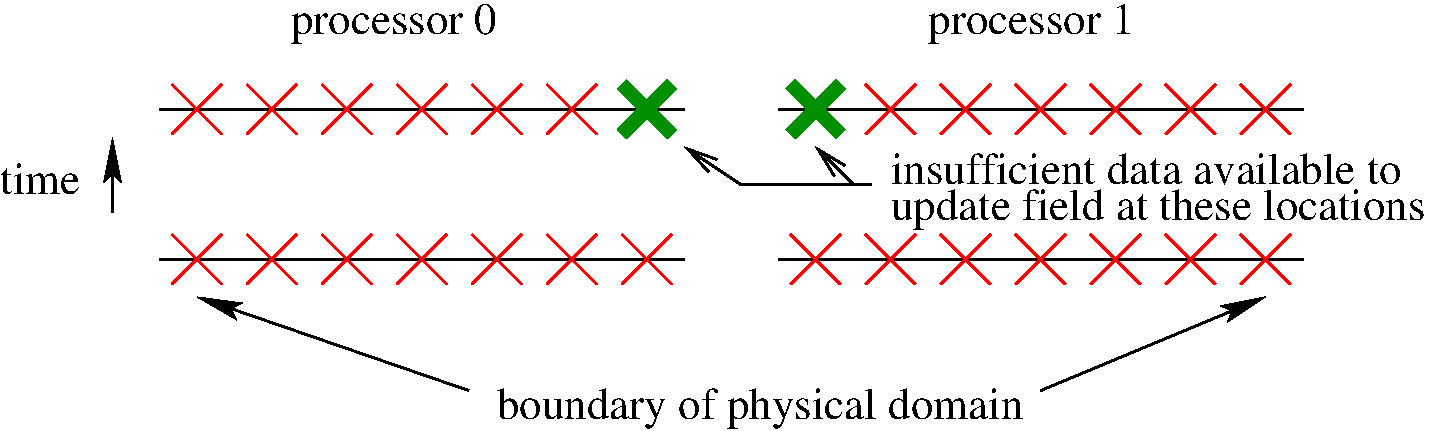
\includegraphics[angle=0,width=8cm]{1dnoghost}
\end{center}
\caption{Distributed wave equation with no ghostzones}
\label{fig:noghost}
\end{figure}

At the outer boundary of the physical domain, the data for the boundary
point can be generated by the boundary conditions, however, at internal
boundaries, the data has to be copied from the adjacent processor.  It
would be inefficient to copy each point individually, so instead, a
number of \textit{ghostzones} are created at the internal boundaries.  A
ghostzone consists of a copy of the whole plane (in 3D, line in 2D,
point in 1D) of the data from the adjacent processor.  That is, the array
on each processor is augmented with copies of points from the adjacent
processors, thus allowing the algorithm to proceed \textit{on the points
owned by this processor} without having to worry about copying data.
Once the data has been evolved one step, the data in the ghostzones
can be exchanged (or \textit{synchronised}) between processors in one
fell swoop before the next evolution step.  (See Figure
\ref{fig:withghost}.)  Note that you should have at least as many
ghostzones as your stencil size requires.

\begin{figure}[ht]
\begin{center}
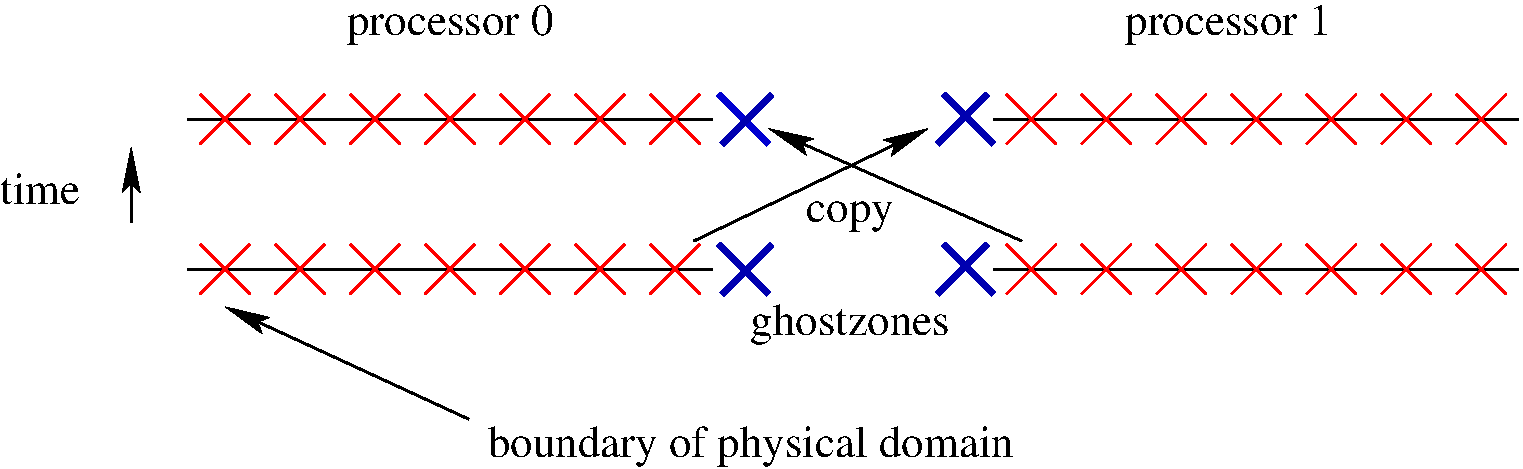
\includegraphics[angle=0,width=8cm]{withghost}
\end{center}
\caption{Distributed wave equation with ghostzones}
\label{fig:withghost}
\end{figure}

%%%%%%%%%%%%%%%%%%%%%%%%%%%%%%%%%%%%%%%%%%%%%%%%%%%%%%%%%%%%%%%%%%%%%%%

\subsection{Information about Grid Variables}

The flesh holds a database with information related to grid variables, and
provides a set of querying APIs.

\subsubsection{Group Information}

Fundamental information about grid functions (e.g.\ local grid size and
location, number of ghostzones) is passed through the argument list of
scheduled routines (see Section~\ref{sec:cactus_variables_c}). To obtain similar information
from non-scheduled routines, or for general grid variables, a set of
functions are provided, the last two letters of which specify whether
the information is requested using a group name (\texttt{GN}) or index
(\texttt{GI}), or a variable name (\texttt{VN}) or index (\texttt{VI}).

\begin{Lentry}

\item [\texttt{CCTK\_Grouplsh[GN|GI|VN|VI]}]    An array of integers
      with the local grid size on this processor.

\item [\texttt{CCTK\_Groupgsh[GN|GI|VN|VI]}]    An array of integers
      with the global grid size.

\item [\texttt{CCTK\_Groupbbox[GN|GI|VN|VI]}]      An array of  integers
      which indicate whether the boundaries are internal boundaries
      (e.g.\ between processors), or physical boundaries.
        A value of \texttt{1} indicates
      a physical (outer) boundary at the edge of the computational grid,
      and \texttt{0} indicates an internal boundary.

\item [\texttt{CCTK\_Groupnghostzones[GN|GI|VN|VI]}]    An array of integers with
         the number of ghostzones used in each direction.

\item [\texttt{CCTK\_Grouplbnd[GN|GI|VN|VI]}]       An array of integers
      containing the lowest index (in each direction)
      of the local grid, as seen on the global grid. Note that these indices
      start from zero, so you need to add one when using them in
      Fortran thorns.

\item [\texttt{CCTK\_Groupubnd[GN|GI|VN|VI]}]       An array of integers
      containing the largest index (in each direction)
      of the local grid, as seen on the global grid. Note that these indices
      start from zero, so you need to add one when using them in
      Fortran thorns.

\end{Lentry}

%%%%%%%%%%%%%%%%%%%%%%%%%%%%%%%%%%%%%%%%%%%%%%%%%%%%%%%%%%%%%%%%%%%%%%%%%%%%%%%
%%%%%%%%%%%%%%%%%%%%%%%%%%%%%%%%%%%%%%%%%%%%%%%%%%%%%%%%%%%%%%%%%%%%%%%%%%%%%%%

\section{Cactus Parameters}
\label{chap:Cactus_parameters}

Parameters are the means by which the user specifies the runtime behaviour of
the code.  Each parameter has a data type and a name, as well as a
range of allowed values and a default value.  These are declared in the thorn's
\texttt{param.ccl} file.

The thorn determines which parameters can be used in other thorns by
specifying a \textit{scope} for the thorn, as explained in Section
\ref{sec:Cactus_parameters.scope}.

The user may specify initial values for parameters in the parameter file
(see Section~\ref{sec:Parameter_File}); the flesh validates these values
against the parameters' allowed ranges.
Otherwise, the initial value of the parameter is taken to be its default.
Once validated, parameter values are fixed, and cannot be changed,
unless the parameter is specified to be \textit{steerable}
(see \ref{sec:Cactus_parameters.steerable}).
For a detailed discussion of the \texttt{param.ccl} syntax, see
Appendix~\ref{sec:Appendix.param}.

The full specification for a parameter declaration is
\begin{alltt}
[EXTENDS|USES] <\var{parameter_type}>[[<\var{size}>]] <\var{parameter name}> "<\var{parameter description}>"
\{
  <\var{PARAMETER_RANGES}>
\} <\var{default value}>
\end{alltt}

You can obtain lists of the parameters associated with
each thorn using the Cactus command line options \texttt{-o} and \texttt{-O}
(Section~\ref{sec:command_line_options}).


%%%%%%%%%%%%%%%%%%%%%%%%%%%%%%%%%%%%%%%%%%%%%%%%%%%%%%%%%%%%%%%%%%%%%%%

\subsection{Types and Ranges}
\label{sec:Parameters.Types_and_Ranges}

Parameters can be of these types:

\begin{Lentry}
\item[Int]  Can take any integral value
\item[Real] Can take any floating point value
\item[Keyword] Can have a value consisting of one of a choice of strings
\item[Boolean] Can be true or false ({\t 1}, {\t t}, {\t true}, or
{\t 0}, {\t f}, {\t false})
\item[String] Can have any string value
\end{Lentry}

Each parameter can be validated against a set of allowed
\textit{ranges}, each of which has a description associated with it.
The nature
of the range is determined by the type of parameter, as follows:

\subsubsection{Int}

The range specification is of the form

\begin{alltt}
\var{lower}:\var{upper}:\var{stride}
\end{alltt}

where \var{lower} and \var{upper} specify the lower and upper allowed
range, and \var{stride} allows numbers to be be missed out, e.g.\
\begin{verbatim}
1:21:2
\end{verbatim}
means the value must be an odd number between one and twenty-one
(inclusive).

A missing end of range (or a `\texttt{*}') indicates negative or positive

Note that if \var{stride} is specified, then \var{upper} must be specified, or `\texttt{*}' (i.e.
the specifier `\texttt{1::2}' is not legal)

infinity, and the default stride is one.
A `\texttt{(}' (or `\texttt{)}') before (or after) the lower (or upper) range specifies an open
endpoint.

\subsubsection{Real}

The range specification is of the form
\begin{alltt}
\var{lower}:\var{upper}
\end{alltt}
where \var{lower} and \var{upper} specify the lower and upper allowed
range.  A missing end of range (or a `\texttt{*}') implies negative or positive
infinity.  The above is inclusive of the endpoints.
A `\texttt{(}' (or `\texttt{)}') before (or after) the lower (or upper) range specifies an open
endpoint.
Likewise, a `\texttt{[} (or `\texttt{]}') before (or after) the lower
(or upper) range specifies a closed endpoint.

The numbers written in a \texttt{param.ccl} file are interpreted as C code.
To express a number in `scientific notation', use,
e.g.\ `\texttt{1e-10}', which is a double precision constant in C.  (If the
floating precision of the variable to which it is assigned is not
double, then C will typecast appropriately.  If you \emph{really} want to
specify a single precision floating constant, or a long double
constant, append the number with {\t f} or {\t l} respectively.)

\subsubsection{Keyword}

The range specification consists of a string, which will be matched in
a case insensitive manner.

\subsubsection{Boolean}

There is no range specification for this type of parameter.

\subsubsection{String}

The range is a POSIX regular expression.  On some machines you may be
able to use extended regular expressions, but this is not guaranteed
to be portable.

%%%%%%%%%%%%%%%%%%%%%%%%%%%%%%%%%%%%%%%%%%%%%%%%%%%%%%%%%%%%%%%%%%%%%%%

\subsection{Scope}
\label{sec:Cactus_parameters.scope}

Parameters can be \texttt{GLOBAL}, \texttt{RESTRICTED}, or \texttt{PRIVATE}.
Global parameters are visible to all thorns.  Restricted parameters
are visible to any thorn which chooses to \texttt{USE} or \texttt{EXTEND}
it.  A private parameter is only visible to the thorn which declares
it.  The default scope is \texttt{PRIVATE}.

\subsection{Steerable}
\label{sec:Cactus_parameters.steerable}
A parameter can be changed dynamically if it is specified to be
\textit{steerable} (see
Section~\ref{subsec:Appendix.param.specification_items}).
It can then be changed by a call to the flesh function
\texttt{CCTK\_ParameterSet} (see the Reference Guide for a description
of this function).

%%%%%%%%%%%%%%%%%%%%%%%%%%%%%%%%%%%%%%%%%%%%%%%%%%%%%%%%%%%%%%%%%%%%%%%%%%%%%%%
%%%%%%%%%%%%%%%%%%%%%%%%%%%%%%%%%%%%%%%%%%%%%%%%%%%%%%%%%%%%%%%%%%%%%%%%%%%%%%%

\section{Scheduling}
\label{chap:scheduling}

Cactus contains a rule-based scheduling system, which determines which
routines, from which thorns are run in which order.  The scheduler
determines if the specifications are inconsistent, but does allow the
user to schedule a routine with respect to another routine which may not
exist.
For a detailed discussion of the {\t schedule.ccl} syntax see
Appendix~\ref{sec:Appendix.schedule}.

A usual simple specification for a schedule declaration is
\begin{alltt}schedule <\var{function name}> AT <\var{schedule bin}>
\{
  LANG: <\var{language}>
  [STORAGE:       <\var{group}>[[\var{timelevels}]],<\var{group}>[[\var{timelevels}]]...]
\} "\var{Description of function}"
\end{alltt}

The full specification for a schedule declaration is
\begin{alltt}schedule [GROUP] <function|\var{schedule group name}> AT|IN <\var{schedule bin}|\var{group name}>
         [AS <\var{alias}>]
         [WHILE <\var{variable}>] [IF <\var{variable}>]
         [BEFORE|AFTER <\var{item}>|(<\var{item}> <\var{item}> ...)]
\{
  LANG: <\var{language}>
  [STORAGE:       <\var{group}>[[\var{timelevels}]],<\var{group}>[[\var{timelevels}]]...]
  [TRIGGER:       <\var{group}>,<\var{group}>...]
  [SYNC:          <\var{group}>,<\var{group}>...]
  [OPTIONS:       <\var{option}>,<\var{option}>...]
\} "\var{Description of function or schedule group}"
\end{alltt}

This full schedule specification consists of a mandatory part, a set
of options, and the main body limited by braces, referred to as the
\texttt{schedule block}.

Each schedule item is scheduled either \texttt{AT} a particular
\var{scheduling bin}, or \texttt{IN} a schedule \var{group}.

%%%%%%%%%%%%%%%%%%%%%%%%%%%%%%%%%%%%%%%%%%%%%%%%%%%%%%%%%%%%%%%%%%%%%%%

\subsection{Schedule Bins}
\label{scheduling:schedule_bins}

These are the main times at which scheduled functions are run, from
fixed points in the flesh and driver thorn (schedule bins can easily
be traversed from any thorn, although this is not usual).  When a
schedule bin is \textit{traversed}, all the functions scheduled in that
particular are called, in the manner described in Section
\ref{scheduling:calling_scheduled_functions} and respecting the
requested ordering of functions(Section~\ref{scheduling:schedule_options}). In the absence of any ordering, functions in a particular schedule bin will be called in
an undetermined order.

The schedule bins are described in Section \ref{subsec:schedule_ccl}. Note that
the preceding \texttt{CCTK\_} is optional for the use of the bin names
in the \texttt{schedule.ccl} file.

%%%%%%%%%%%%%%%%%%%%%%%%%%%%%%%%%%%%%%%%%%%%%%%%%%%%%%%%%%%%%%%%%%%%%%%

\subsection{Groups}
\label{scheduling:groups}

If the optional \texttt{GROUP} specifier is used, the item is a schedule
group rather than a normal function.  Schedule groups are effectively
new, user-defined, schedule bins.  Functions or groups may be
scheduled \texttt{IN} these, in the same way as they are scheduled {\tt
AT} the main schedule bins.  (That is, groups may be nested.)

%%%%%%%%%%%%%%%%%%%%%%%%%%%%%%%%%%%%%%%%%%%%%%%%%%%%%%%%%%%%%%%%%%%%%%%

\subsection{Schedule Options}
\label{scheduling:schedule_options}
The options define various characteristics of the schedule item.

\begin{Lentry}
\item[\texttt{AS}]
This assigns a new name to a function for scheduling purposes.  This
is used, for instance, to allow a thorn to schedule something before
or after a routine from another implementation;  two thorns providing this
implementation can schedule a routine \texttt{AS} the same thing, thus
allowing other thorns to operate independently of which one is active.

\item[\texttt{WHILE}]
This specifies a \texttt{CCTK\_INT} grid scalar which is used to
control the execution of this item.  As long as the grid scalar has
a nonzero value, the schedule item will be executed repeatedly.  This
allows dynamic behaviour with scheduling.

\item[\texttt{IF}]
This specifies a \texttt{CCTK\_INT} grid scalar which is used to
control the execution of this item.  If the grid scalar has a
nonzero value, the schedule item will be executed, otherwise the item
will be ignored.  This allows dynamic behaviour with scheduling.

If both an \texttt{IF} and a \texttt{WHILE} clause are present, then
the schedule is executed according to the following pseudocode:
\begin{verbatim}
IF condition
  WHILE condition
    SCHEDULE item
  END WHILE
END IF
\end{verbatim}

\item[\texttt{BEFORE} or \texttt{AFTER}]
These specify either
\begin{itemize}
\item   a function or group before or after which this item will be
        scheduled, or
\item   a list of functions and/or groups; this item will be scheduled
        (once) before any of them or after all of them respectively.
\end{itemize}
Note that a single schedule item may have multiple \texttt{BEFORE}
and/or \texttt{AFTER} options; the scheduler will honor all of these
(or abort with a fatal error).  For example,
\begin{alltt}
schedule FOO BEFORE A BEFORE B BEFORE C ...
\end{alltt}
schedules \texttt{FOO} before any of \texttt{A}, \texttt{B}, or \texttt{C}.
This can also be written
\begin{alltt}
schedule FOO BEFORE (A B C) ...
\end{alltt}

Note that the set of all \texttt{BEFORE}/\texttt{AFTER} options in
all active schedule blocks of all active thorns, \emph{must} specify
a (directed) graph with no cycles; if there are any cycles, then the
scheduler will abort with a fatal error.
\end{Lentry}

%%%%%%%%%%%%%%%%%%%%%%%%%%%%%%%%%%%%%%%%%%%%%%%%%%%%%%%%%%%%%%%%%%%%%%%

\subsection{The Schedule Block}
\label{scheduling:schedule_block}

The schedule block specifies further details of the scheduled function
or group.

\begin{Lentry}
\item[\texttt{LANG}]
This specifies the language of the routine.  Currently this is either
C or Fortran. C++ routines should be defined as \texttt{extern "C"}
and registered as \texttt{LANG: C}.
\item[\texttt{STORAGE}] The \texttt{STORAGE} keyword specifies groups for
which memory should be allocated for the duration of the routine or
schedule group.  The storage status reverts to its previous status
after completion of the routine or schedule group.
Each group must specify how many timelevels to activate storage for,
from 1 up to the maximum number for the group as specified in the
defining {\tt interface.ccl} file. If the maximum is 1 (the default)
this number may be omitted. Alternatively \var{timelevels} can be the
name of a parameter accessible to the thorn. The parameter name is the
same as used in C routines of the thorn, fully qualified parameter names
of the form \texttt{\var{thorn}::\var{parameter}} are not allowed. In this
case 0 (zero) \var{timelevels} can be requested, which is equivalent to
the {\tt STORAGE} statement being absent.

\item[\texttt{TRIGGER}]
This is only used for items scheduled at timebin \texttt{CCTK\_ANALYSIS}.
The item will only be executed if output is due for at least one
variable in one of the listed groups.  (The item will also be called
if there is no group listed.)
\item[\texttt{SYNC}]
On exit from this item, the ghost zones of the listed groups will be
exchanged.
\item[\texttt{OPTIONS}]
This is for miscellaneous options.  The list of accepted options is
given in Appendix~\ref{app:allopts}.
\end{Lentry}

%%%%%%%%%%%%%%%%%%%%%%%%%%%%%%%%%%%%%%%%%%%%%%%%%%%%%%%%%%%%%%%%%%%%%%%

\subsection{How Cactus Calls Scheduled Functions}
\label{scheduling:calling_scheduled_functions}

For each scheduled function called, the flesh performs a variety of jobs
at entry and exit.

On entry to a scheduled routine, if the routine is being called at the
\texttt{CCTK\_ANALYSIS} timebin first, a check is made to see if the routine should
actually be called on this timestep. For this, all grid variables in the
trigger groups for the routine are checked with all registered output
methods to determine if it is time to output any triggers. The routine
will only be called if at least one is due to be output. Note that once
a grid variable has been analyzed, it gets marked as such, and will not
be analyzed again during this iteration.
(Note that a routine without any trigger groups will also be called.)
Thus, if more than one analysis
routine should be triggered on the same trigger variable(s), they must
be scheduled in a single group. Routines from all timebins, other than \texttt{ANALYSIS}, are always called.

Next, storage is assigned for any required variables, remembering the
original state of storage.

The routine is then called, and on exit, any required grid variables are
first synchronised. Following synchronization, any required output methods
are called for the triggers. Finally, the storage of grid variables is
returned to the original state.

%%%%%%%%%%%%%%%%%%%%%%%%%%%%%%%%%%%%%%%%%%%%%%%%%%%%%%%%%%%%%%%%%%%%%%%%%%%%%%%
%%%%%%%%%%%%%%%%%%%%%%%%%%%%%%%%%%%%%%%%%%%%%%%%%%%%%%%%%%%%%%%%%%%%%%%%%%%%%%%

\section{Writing a Thorn}

%%%%%%%%%%%%%%%%%%%%%%%%%%%%%%%%%%%%%%%%%%%%%%%%%%%%%%%%%%%%%%%%%%%%%%%

\subsection{Thorn Programming Languages}

When you start writing a new thorn, the first decision to make is
which programming language to use. The source code in Cactus thorns
can be written in any mixture of C, C++, CUDA, or Fortran.
The following points should be considered when
choosing a language to work in:
\begin{itemize}

\item All functions designed for application thorn writers are available
      in all languages, however, some interfaces for infrastructure
      thorn writing are only available from C or C++.

\end{itemize}

Whatever language you choose, if you want your thorn to be portable, and
compile and run on multiple platforms, stick to the standards and don't
use machine dependent extensions.

%%%%%%%%%%%%%%%%%%%%%%%%%%%%%%%%%%%%%%%%%%%%%%%%%%%%%%%%%%%%%%%%%%%%%%%

\subsection{What the Flesh Provides}

The flesh provides for thorns:
\begin{Lentry}
\item [\texttt{Variables}]
\item [\texttt{Parameters}]
\item [\texttt{Cactus Functions}]

\begin{itemize}
  \item{} Driver (parallelisation) utilities
  \item{} I/O utilities
  \item{} Coordinates utilities
  \item{} Reduction utilities
  \item{} Interpolation utilities
  \item{} Information utilities
\end{itemize}
\end{Lentry}


\subsubsection{Fortran Routines}

Any source file using Cactus infrastructure should include
the header file \texttt{cctk.h} using the line
\begin{verbatim}
#include "cctk.h"
\end{verbatim}
(Fortran programmers should not be put off by this being a C style
header file---most Cactus files are run through a C preprocessor
before compilation.)

\paragraph{Variables}

Any routine using Cactus argument lists (for example, all routines called from
the scheduler at time bins between {\t CCTK\_STARTUP} and {\t CCTK\_SHUTDOWN})
should include at the top of the file the header
\begin{verbatim}
#include "cctk_Arguments.h"
\end{verbatim}

A Cactus macro \texttt{CCTK\_ARGUMENTS} is defined for each thorn
to contain:
\begin{itemize}
\item General information about the grid hierarchy, for example, the number
      of grid points used. See Section \ref{sec:cactus_variables_c} for a
      complete list.
\item All the grid variables defined in the thorn's \texttt{interface.ccl}
\item All the grid variables required from other thorns as requested by
      the \texttt{inherits} and \texttt{friend} lines in the \texttt{interface.ccl}
\end{itemize}
These variables must be declared at the start of the routine using
the macro \texttt{DECLARE\_CCTK\_ARGUMENTS}. Alternatively, they can
be declared with \texttt{DECLARE\_CCTK\_ARGUMENTS\_CHECKED(<function name>}),
where \texttt{<function name>} is the name of the function as declared
in \texttt{schedule.ccl}. The function-name specific version of the macro
will declare only those variables identified by READS/WRITES directives
in \texttt{schedule.ccl}, using \texttt{const} for the C/C++ variables
and \texttt{intent(in)} for the Fortran variables. (Note that, for technical
reasons, in Fortran variables declared in \texttt{DECLARE\_CCTK\_ARGUMENTS}
but not in the \texttt{READS/WRITES} directives are actually declared as
\texttt{intent(in), character*8}, and are thus unusable.)

To pass the arguments to another routine in the same thorn use the macro
\texttt{CCTK\_PASS\_FTOF} in the calling routine, and again the macro
\texttt{CCTK\_ARGUMENTS} in the receiving routine.

Note that you cannot use Cactus argument lists in routines scheduled at the
{\t CCTK\_STARTUP} and {\t CCTK\_SHUTDOWN} time bins, because at this time
no grid hierarchy exists.


\paragraph{Parameters}

All parameters defined in a thorn's \texttt{param.ccl} and all \texttt{global}
parameters, appear as local variables of the corresponding \texttt{CCTK} data type
in Fortran source code, i.e. Booleans and Integers appear as \texttt{CCTK\_INT}
types (with nonzero/zero values for boolean {\t yes/no}),
Reals as \texttt{CCTK\_REAL}, and Keywords and String parameters as
\texttt{CCTK\_STRING} (see
also note below). These variables are \emph{read only}, and \emph{changes should
not be made to them}. The effect of changing a parameter is undefined (at best).

Any routine using Cactus parameters should include at
the top of the file the header
\begin{verbatim}
#include "cctk_Parameters.h"
\end{verbatim}

The parameters should be declared at the start of the routine
using them with the macro \texttt{DECLARE\_CCTK\_PARAMETERS}.

In Fortran, special care should be taken with string valued parameters.
These parameters are passed as C pointers, and can not be treated as
normal Fortran strings.
To compare a string valued parameter and Fortran
string, use the macro \texttt{CCTK\_EQUALS()} or the function \texttt{CCTK\_Equals()}
(see the reference manual for a description of the \texttt{CCTK\_} functions).
To print the value of a string valued parameter to screen, use the subroutine
\texttt{CCTK\_PrintString()}. A further function \texttt{CCTK\_FortranString}
provides a mechanism for converting a string parameter to a Fortran string.
For example, if \texttt{operator} is a Cactus string parameter holding the name of a reduction operator whose handle you need to find, you cannot pass it
directly into the subroutine \texttt{CCTK\_LocalArrayReductionHandle}, which is expecting
a Fortran string. Instead, the following is needed:
%
\begin{verbatim}
      character*200 fortran_operator
      CCTK_INT      fortran_operator_len
      integer       handle

      call CCTK_FortranString(fortran_operator_len,operator,fortran_operator)
      call CCTK_LocalArrayReductionHandle(handle,fortran_operator(1:fortran_operator_len))
\end{verbatim}



\paragraph{Fortran Example}

The Fortran routine, \verb|MyFRoutine|, is scheduled in the {\tt
schedule.ccl} file, doesn't use Cactus parameters, and calls another
routine, in the same thorn, \verb|MyNewRoutine|, which does use
parameters.  This routine needs to be passed an integer flag as well
as the standard Cactus variables. The source file should look like
%
\begin{verbatim}
#include "cctk.h"
#include "cctk_Arguments.h"
#include "cctk_Parameters.h"

      subroutine MyFRoutine(CCTK_ARGUMENTS)

c     I'm very cautious, so I want to declare all variables
      implicit none

      DECLARE_CCTK_ARGUMENTS_CHECKED(MyFRoutine)
c Note: It is also possible to use
c     DECLARE_CCTK_ARGUMENTS
c However, this latter form will declare all variables
c available to the thorn and not simply those listed
c in the READS/WRITES clauses of the schedule.ccl declaration.
c
c Note: It is also possible to use all caps for the function
c name when writing in Fortran. Thus, the following also works:
c
c     DECLARE_CCTK_ARGUMENTS_CHECKED(MYFROUTINE)

      integer flag

      flag = 1
      call MyNewRoutine(CCTK_PASS_FTOF,flag)

      return
      end

      subroutine MyNewRoutine(CCTK_ARGUMENTS,flag)

      implicit none

      DECLARE_CCTK_ARGUMENTS_CHECKED(MyNewRoutine)
      DECLARE_CCTK_PARAMETERS
      integer flag

c     Main code goes here

      return
      end

\end{verbatim}

\paragraph{Cactus Fortran Functions}

Cactus Fortran functions, for example, \texttt{CCTK\_MyProc} and {\tt
CCTK\_Equals}, can all be declared by adding the statement
%
\begin{verbatim}
#include "cctk_Functions.h"
\end{verbatim}
%
near the top of the file, and adding the declaration
%
\begin{verbatim}
DECLARE_CCTK_FUNCTIONS
\end{verbatim}
%
to a module or a subroutine after the \texttt{implicit none}
statement, but before any executable code.

\paragraph{Fortran Modules}
\label{par:fortran_modules}

Fortran modules should be placed into source files that have the same
name as the module, followed by the corresponding file name suffix.  A
module \texttt{metric} should thus be placed, e.g.\ into a file
\texttt{metric.F90}.  This convention allows the Cactus build system
to automatically deduce the compile time dependencies.

If you do not follow this convention, then you have to include the
modules into the thorn's \texttt{make.code.deps} file
(Section \ref{sec:mabathbu}) to ensure they are compiled before the routines
which use them.  This is especially important for parallel building.
For example, if a routine in \texttt{MyRoutine.F90} uses a module in {\tt
MyModule.F90}, then add the line:
%
\begin{verbatim}
MyRoutine.F90.o:         MyModule.F90.o
\end{verbatim}

\paragraph{The \texttt{MOD} function}

The intrinsic function \texttt{MOD} in Fortran takes two integer
arguments, which should both be of the same type. This means
that it may be necessary to cast the arguments to, e.g.
\texttt{INT} for some architectures. This can occur in particular
when a \texttt{CCTK\_INT} parameter and the Cactus variable \texttt{cctk\_iteration}
(which is declared to be \texttt{INTEGER}) are used,
in which case the correct code is
\begin{verbatim}
MOD(cctk_iteration,INT(MyParameter))
\end{verbatim}


\subsubsection{C Routines}

Any source file using Cactus infrastructure should include
the header file \texttt{cctk.h} using the line
\begin{verbatim}
#include "cctk.h"
\end{verbatim}

\paragraph{Variables}

Any routine using Cactus argument lists (for example, all routines called from
the scheduler at time bins between {\t CCTK\_STARTUP} and {\t CCTK\_SHUTDOWN}),
should include at the top of the file the header
\begin{verbatim}
#include "cctk_Arguments.h"
\end{verbatim}

A Cactus macro \texttt{CCTK\_ARGUMENTS} is defined for each thorn
to contain
\begin{itemize}
\item General information about the grid hierarchy, for example, the
number of grid points on the processor. See Section \ref{sec:cactus_variables_c}
for a complete list.
\item All the grid variables defined in the thorn's \texttt{interface.ccl}
\item All the grid variables required from other thorns as requested by
      the \texttt{inherits} and \texttt{friend} lines in the \texttt{interface.ccl}
\end{itemize}
These variables must be declared at the start of the routine using
the macro \texttt{DECLARE\_CCTK\_ARGUMENTS}. This macro should always be the
first line of the routine.

To pass the arguments to another routine in the same thorn, use the macro
\texttt{CCTK\_PASS\_CTOC} in the calling routine, and again the macro
\texttt{CCTK\_ARGUMENTS} in the receiving routine.

Note that you cannot use Cactus argument lists in routines scheduled at the
{\t CCTK\_STARTUP} and {\t CCTK\_SHUTDOWN} time bins, because at this time
no grid hierarchy exists.


\paragraph{Parameters}

All parameters defined in a thorn's \texttt{param.ccl} and all \texttt{global}
parameters, appear as local variables of the corresponding \texttt{CCTK} data type
in C source code, i.e. Integers and Booleans appear as \texttt{CCTK\_INT} types
(with nonzero/zero values for boolean {\t yes/no}), Reals as
\texttt{CCTK\_REAL}, and Keywords and String parameters as \texttt{CCTK\_STRING}.
These variables are \emph{read only}, and \emph{changes should not be made to
them}.  The effect of changing a parameter is undefined (at best).

Any routine using Cactus parameters should include at
the top of the file the header
\begin{verbatim}
#include "cctk_Parameters.h"
\end{verbatim}

The parameters should be declared as the last statement in the declaration part
of the routine using them with the macro \texttt{DECLARE\_CCTK\_PARAMETERS}.

\paragraph{Example}

The C routine \verb|MyCRoutine| is scheduled in the \texttt{schedule.ccl} file,
and uses Cactus parameters. The source file should look like
\begin{verbatim}
#include "cctk.h"
#include "cctk_Arguments.h"
#include "cctk_Parameters.h"

void MyCRoutine(CCTK_ARGUMENTS)
{
  DECLARE_CCTK_ARGUMENTS_CHECKED(MyCRoutine)
  DECLARE_CCTK_PARAMETERS

  /* Here goes your code */
}
\end{verbatim}

\paragraph{Complex variables}

Cactus supports complex grid variables of type \texttt{CCTK\_COMPLEX} which
are realized through the types \texttt{complex}, \texttt{std::complex} and
\texttt{COMPLEX} in C, C++ and Fortran respectively. Complex number support is
available in C in the C99 language standard which Cactus requires.

There is a known incompatibility when \emph{returning} complex numbers from C
and Fortran functions to C++ callers on some architectures. Access to
variables through pointers and in arrays is not affected. A workaround is not
to return values but instead pass in a pointer to a local variable to hold the
return value.

\paragraph{Specifically for C Programmers}

Grid functions are held in memory as 1-dimensional C arrays. These are laid
out in memory as in Fortran. This means that the first index should
be incremented through most rapidly.  This is illustrated in the example
below.

Cactus provides
macros to find the 1-dimensional index which is needed from the multidimensional
indices which are usually used. There is a macro for each dimension of
grid function.  Below is an artificial example to demonstrate this
using the 3D macro \texttt{CCTK\_GFINDEX3D}:
\begin{verbatim}
for (k=0; k<cctk_lsh[2]; k++)
{
  for (j=0; j<cctk_lsh[1]; j++)
  {
    for (i=0; i<cctk_lsh[0]; i++)
    {
      int const ind3d = CCTK_GFINDEX3D(cctkGH,i,j,k);
      rho[ind3d] = exp(-pow(r[ind3d],2));
    }
  }
}
\end{verbatim}
%
Here, \verb|CCTK_GFINDEX3D(cctkGH,i,j,k)| expands to
\begin{verbatim}
((i) + cctkGH->cctk_lsh[0]*((j)+cctkGH->cctk_lsh[1]*(k)))
\end{verbatim}
%
Note: In Fortran, grid functions are accessed as Fortran arrays,
i.e.\ simply as \verb|rho(i,j,k)|.

To access vector grid functions (vector grid functions are a
``vector'' of grid functions; see section
\ref{subsec:Appendix.interface-variables}), one also needs to specify
the vector index. This is best done via the 3D macro
\texttt{CCTK\_VECTGFINDEX3D}:
\begin{verbatim}
for (k=0; k<cctk_lsh[2]; k++)
{
  for (j=0; j<cctk_lsh[1]; j++)
  {
    for (i=0; i<cctk_lsh[0]; i++)
    {
      /* vector indices are 0, 1, 2 */
      vel[CCTK_VECTGFINDEX3D(cctkGH,i,j,k,0)] = 1.0;
      vel[CCTK_VECTGFINDEX3D(cctkGH,i,j,k,1)] = 0.0;
      vel[CCTK_VECTGFINDEX3D(cctkGH,i,j,k,2)] = 0.0;
    }
  }
}
\end{verbatim}

\subsubsection{Cactus Variables}
\label{sec:cactus_variables_c}

The Cactus variables which are passed through the macro
\texttt{CCTK\_ARGUMENTS} are
\begin{Lentry}
\item [\texttt{cctkGH}] A C pointer identifying the grid hierarchy.
\item [\texttt{cctk\_dim}] An integer with the number of dimensions
      used for this grid hierarchy.
\item [\texttt{cctk\_lsh}] An array of \texttt{cctk\_dim} integers
      with the local grid size on this processor.
\item [\texttt{cctk\_ash}] An array of \texttt{cctk\_dim} integers
      with the allocated size of the array.  This may be larger than
      the local size; the additional points may not be used.
\item [\texttt{cctk\_gsh}] An array of \texttt{cctk\_dim} integers
      with the \textit{global} grid size.
\item [\texttt{cctk\_iteration}] The current iteration number.
\item [\texttt{cctk\_delta\_time}] A \texttt{CCTK\_REAL} with the timestep.
\item [\texttt{cctk\_time}] A \texttt{CCTK\_REAL} with the current time.
\item [\texttt{cctk\_delta\_space}] An array of \texttt{cctk\_dim} {\tt
CCTK\_REAL}s with the grid spacing in each direction.
\item [\texttt{cctk\_nghostzones}] An array of \texttt{cctk\_dim} integers with
         the number of ghostzones used in each direction.
%\item [\texttt{cctk\_from}] The index value from which the user should start loops.
%\item [\texttt{cctk\_to}] ... end loops.
\item [\texttt{cctk\_origin\_space}] An array of \texttt{cctk\_dim} {\tt
      CCTK\_REAL}s with the spatial coordinates of the global origin
      of the grid.

\end{Lentry}

The following variables describe the location of the local
grid (e.g.\ the grid treated on a given processor) within
the global grid.
\begin{Lentry}
\item [\texttt{cctk\_lbnd}]
      An array of \texttt{cctk\_dim} integers
      containing the lowest index (in each direction)
      of the local grid, as seen on the global grid. Note that these indices
      start from zero, so you need to add one when using them in
      Fortran thorns.
\item [\texttt{cctk\_ubnd}]
      An array of \texttt{cctk\_dim} integers
      containing the largest index (in each direction)
      of the local grid, as seen on the global grid.  Note that these indices
      start from zero, so you need to add one when using them in
      Fortran thorns.
\item [\texttt{cctk\_bbox}]
      An array of 2$*$\texttt{cctk\_dim} integers (in the order
        $[\mbox{dim}_0^{\mbox{min}}, \mbox{dim}_0^{\mbox{max}},
        \mbox{dim}_1^{\mbox{min}}, \mbox{dim}_1^{\mbox{max}}, \ldots]$),
      which indicate whether the boundaries are internal boundaries
      (e.g.\ between processors), or physical boundaries.
      A value of 1 indicates
      a physical (outer) boundary at the edge of the computational grid,
      and 0 indicates an internal boundary.
\end{Lentry}

The following variable is needed for grid refinement methods
\begin{Lentry}
\item [\texttt{cctk\_levfac}] An array of \texttt{cctk\_dim} integer factors
        by which the local grid is refined in the corresponding
        direction with respect to the base grid.
\item [\texttt{cctk\_levoff}] and \texttt{cctk\_levoffdenom} Two arrays of
        \texttt{cctk\_dim} integers describing the distance by which the
        local grid is offset with respect to the base grid, measured
        in local grid spacings.  The distance in direction \texttt{dir}
        is given by \texttt{1.0 * cctk\_levoff[dir] /
        cctk\_levoffdenom[dir]}.
\item [\texttt{cctk\_timefac}] The integer factor
        by which the time step size is reduced with respect to the
        base grid.
\end{Lentry}

The following variables are used for identifying convergence levels.

\begin{Lentry}
\item [\texttt{cctk\_convlevel}] The convergence level of this grid hierarchy.
        The base level is $0$, and every level above that is
        coarsened by a factor of \texttt{cctk\_convfac}.
\item [\texttt{cctk\_convfac}] The factor between convergence levels.
        The relation between the resolutions of different convergence
        levels is $\Delta x_L = \Delta x_0 \cdot F^L$, where $L$ is the
        convergence level and $F$ is the convergence factor.
        The convergence factor defaults to $2$.
\end{Lentry}

The variables \texttt{cctk\_delta\_space}, \texttt{cctk\_delta\_time}, and
\texttt{cctk\_origin\_space} denote the grid spacings, time step size,
and spatial origin on the \textit{base} grid.  If you are using a grid
refinement method, you need to calculate these quantities on the grid
you are on.  There are Cactus macros provided for this, with the
syntax \texttt{CCTK\_DELTA\_SPACE(dir)}, \texttt{CCTK\_ORIGIN\_SPACE(dir)},
and \texttt{CCTK\_DELTA\_TIME} for both C and Fortran.  It is recommended
that these macros are always used to provide the grid spacings, time
step sizes, and spatial origins in your thorns.  In doing so, you
incorporate the effects of \texttt{cctk\_levfac}, \texttt{cctk\_levoff},
\texttt{cctk\_levoffdenom}, and \texttt{cctk\_timefac}, so that you do not
explicitly have to take them into account.

Putting the above information together, Figure~\ref{fig-global-xyz-coords}
shows two different ways to compute the global Cactus $xyz$ coordinates
of the current grid point.  Because the ``alternate calculation'' (the
one using \verb|Grid::x|, \verb|Grid::y|, and \verb|Grid::z|) gives the
true global $xyz$ coordinates even in a multipatch/multiblock context,
this is generally the preferred form for general use.

\begin{figure}[bp]
\begin{verbatim}
#include <stddef.h>                     /* defines size_t */
#include "cctk.h"

void MyThorn_MyFunction(CCTK_ARGUMENTS)
{
int i,j,k;

    for (k = 0 ; k < cctk_lsh[2] ; ++k)
    {
    for (j = 0 ; j < cctk_lsh[1] ; ++j)
    {
    for (i = 0 ; i < cctk_lsh[0] ; ++i)
    {
    const size_t posn = CCTK_GFINDEX3D(cctkGH, i,j,k);

    /* calculate the global xyz coordinates of the (i,j,k) grid point */
    /* (in a multipatch/multiblock context, this gives the per-patch coordinates) */
    const CCTK_REAL xcoord = CCTK_ORIGIN_SPACE(0) + (cctk_lbnd[0] + i)*CCTK_DELTA_SPACE(0);
    const CCTK_REAL ycoord = CCTK_ORIGIN_SPACE(1) + (cctk_lbnd[1] + j)*CCTK_DELTA_SPACE(1);
    const CCTK_REAL zcoord = CCTK_ORIGIN_SPACE(2) + (cctk_lbnd[2] + k)*CCTK_DELTA_SPACE(2);

    /* an alternate calculation, which requires that this thorn inherit from  Grid */
    /* (in a multipatch/multiblock context, this gives the true global xyz coordinates) */
    const CCTK_REAL xxcoord = /* Grid:: */ x[posn];
    const CCTK_REAL yycoord = /* Grid:: */ y[posn];
    const CCTK_REAL zzcoord = /* Grid:: */ z[posn];
    }
    }
    }
}
\end{verbatim}
\caption{%%%
	This figure shows two different ways to compute the global
	Cactus $xyz$ coordinates of the current grid point.  Because
	the ``alternate calculation'' (the one one using \texttt{Grid::x},
	\texttt{Grid::y}, and \texttt{Grid::z}) gives the true global
	$xyz$ coordinates even in a multipatch/multiblock context,
	this is generally the preferred form for general use.
	}
\label{fig-global-xyz-coords}
\end{figure}

\subsubsection{Cactus Data Types}

To provide portability across platforms, the Cactus grid variables and parameters are defined and
declared using Cactus data types. The most important of
these data types are described below, for a full description
see Section~\ref{sec:datyansi}. These data types should
be used to declare local variables where needed, and to
declare Cactus grid variables or parameters that need
declarations.

\begin{Lentry}

\item[\texttt{CCTK\_INT}] default size 4 bytes
\item[\texttt{CCTK\_REAL}] default size 8 bytes
\item[\texttt{CCTK\_COMPLEX}] consists of two \texttt{CCTK\_REAL} elements

\end{Lentry}

\paragraph{Example}

In the following example, \verb|MyScalar| is a grid scalar which
is declared in the \texttt{interface.ccl} as \texttt{CCTK\_REAL}.
%
\begin{verbatim}
      subroutine InitialData(CCTK_ARGUMENTS)

      DECLARE_CCTK_ARGUMENTS

      CCTK_REAL local_var

      local_var = 1.0/3.0
      MyScalar = local_var

      return
      end
\end{verbatim}
%
Declaring \texttt{local\_var} to have a non-Cactus data type, e.g.\
\texttt{REAL*4}, or using one of the other Cactus real data types
described in Section~\ref{sec:datyansi}, could give problems for
different architectures or configurations.

%%%%%%%%%%%%%%%%%%%%%%%%%%%%%%%%%%%%%%%%%%%%%%%%%%%%%%%%%%%%%%%%%%%%%%%

\subsection{Parallelisation}
\label{sec:parallelisation}

The flesh itself does not actually set up grid variables. This
is done by a \textit{driver} thorn. To allow the distribution of
a grid over a number of processors, the driver thorn must
also provide the grid decomposition, and routines to enable
parallelisation. The method used to provide this parallelisation
(e.g.\ MPI, PVM) is not usually important for the thorn writer, since
the driver thorn provides routines which are called by standard interfaces
from the flesh. Here, we describe briefly the most important of these routines
for the application thorn writer. A more detailed description
of these interfaces with their arguments, is given in the Reference Manual.
A complete description of the
routines that a driver thorn must provide, will be provided in the
Infrastructure Thorn Writers Guide (Part \ref{chap:infrastructure}). The standard driver thorn is
currently \texttt{PUGH} in the \texttt{CactusPUGH} package, which
is a parallel unigrid driver.

\begin{Lentry}
\item[\texttt{CCTK\_nProcs}] Returns the number of processors being used
\item[\texttt{CCTK\_MyProc}] Returns the processor number (this starts at
  processor number zero)
\item[\texttt{CCTK\_SyncGroup, CCTK\_SyncGroupsI}] Synchronises either a single
  group or a set of groups of grid arrays by
  exchanging the values held in each processor ghostzones, with the
  physical values of their neighbours (see the Reference Manual)
\item[\texttt{CCTK\_Barrier}] Waits for all processors to reach this point
  before proceeding
\end{Lentry}

%%%%%%%%%%%%%%%%%%%%%%%%%%%%%%%%%%%%%%%%%%%%%%%%%%%%%%%%%%%%%%%%%%%%%%%%%%%%%%%
%%%%%%%%%%%%%%%%%%%%%%%%%%%%%%%%%%%%%%%%%%%%%%%%%%%%%%%%%%%%%%%%%%%%%%%%%%%%%%%

\section{Cactus Application Interfaces}

%%%%%%%%%%%%%%%%%%%%%%%%%%%%%%%%%%%%%%%%%%%%%%%%%%%%%%%%%%%%%%%%%%%%%%%

\subsection{Iterating Over Grid Points}
\label{sec:CactusAPI.gridpoints}

A grid function consists of a multi-dimensional array of grid points.
These grid points fall into several types:
\begin{description}
\item[interior] regular grid point, presumably evolved in time
\item[ghost] inter-process boundary, containing copies of values owned
  by another process
\item[physical boundary] outer boundary, presumably defined via a
  boundary condition
\item[symmetry boundary] defined via a symmetry, e.g.\ a reflection
  symmetry or periodicity
\end{description}
Grid points in the edges and corners may combine several types. For
example, a point in a corner may be a ghost point in the $x$
direction, a physical boundary point in the $y$ direction, and a
symmetry point in the $z$ direction.

The size of the physical boundary depends on the application. The
number of ghost points is defined by the driver; the number of
symmetry points is in principle defined by the thorn implementing the
respective symmetry condition, but will in general be the same as the
number of ghost points to avoid inconsistencies.

When iterating over grid points, one usually needs to know about the
boundary sizes and boundary types present. Details about this is
explained in thorn CactusBase/CoordBase.

The flesh provides a set of macros to iterate over particular types of
grid points:
\begin{description}
\item[\texttt{CCTK\_LOOP\_ALL}] Loop over all grid points
\item[\texttt{CCTK\_LOOP\_INT}] Loop over all interior grid points
\item[\texttt{CCTK\_LOOP\_BND}] Loop over all physical boundary points
\item[\texttt{CCTK\_LOOP\_INTBND}] Loop over all ``interior'' physical
  boundary points, i.e.\ over all those physical boundary points that
  are not also ghost or symmetry points
\end{description}

As described above, points on edges and corners can have several
boundary types at once, e.g.\ can be both a physical and a symmetry
point. \texttt{LOOP\_BND} and \texttt{LOOP\_INTBND} treat these
different: \texttt{LOOP\_BND} loops over all points that are physical
boundaries (independent of whether they also are symmetry or ghost
boundaries), while \texttt{LOOP\_INTBND} loops over those points that
are only physical boundaries (and excludes any points that belongs to
a symmetry or ghost boundary). \texttt{LOOP\_BND} does not require
applying a symmetry condition or synchronisation afterwards (but does
not allow taking tangential derivatives); \texttt{LOOP\_INTBND} allows
taking tangential derivatives (but requires applying symmetry
boundaries and synchronising afterwards).

In 3 dimensions, these macros should be called as follows:
\begin{verbatim}
CCTK_LOOP3_ALL(name, cctkGH, i,j,k) {
  ... body of the loop
} CCTK_ENDLOOP3_ALL(name);
\end{verbatim}

\begin{verbatim}
CCTK_LOOP3_INT(name, cctkGH, i,j,k) {
  ... body of the loop
} CCTK_ENDLOOP3_INT(name);
\end{verbatim}

\begin{verbatim}
CCTK_LOOP3_BND(name, cctkGH, i,j,k, ni,nj,nk) {
  ... body of the loop
} CCTK_ENDLOOP3_BND(name);
\end{verbatim}

\begin{verbatim}
CCTK_LOOP3_INTBND(name, cctkGH, i,j,k, ni,nj,nk) {
  ... body of the loop
} CCTK_ENDLOOP3_INTBND(name);
\end{verbatim}
and similarly for 2 dimensions and 1 dimension.

In all cases, \texttt{name} should be replaced by a unique name for
the loop. \texttt{i}, \texttt{j}, and \texttt{k} are names of
variables that will be declared and defined by these macros,
containing the index of the current grid point. Similarly \texttt{ni},
\texttt{nj}, and \texttt{nk} are names of variables describing the
(outwards pointing) normal direction to the boundary as well as the
distance to the boundary.

\paragraph{\texttt{OpenMP}} All \texttt{CCTK\_LOOP} macros include support for
\texttt{OpenMP} based multi-threading when called inside of an \texttt{OpenMP}
parallel section. They do no themselves create such a parallel section and
therefore should be preceded by a \texttt{\#pragma omp parallel}:
\begin{verbatim}
#pragma omp parallel
CCTK_LOOP3_ALL(name, cctkGH, i,j,k) {
  ... body of the loop
} CCTK_ENDLOOP3_ALL(name);
\end{verbatim}
and similar for \texttt{CCTK\_LOOP3\_INT}, \texttt{CCTK\_LOOP3\_BND}, and
\texttt{CCTK\_LOOP3\_INTBND}.

\subsection{Coordinates}
\label{sec:CactusAPI.coordinates}

The flesh provides utility routines for registering and querying
coordinate information. The flesh does not provide any coordinates
itself, these must be supplied by a thorn. Thorns are not required to
register coordinates to the flesh, but registering coordinates
provides a means for infrastructure thorns to make use of coordinate
information.

Coordinates are grouped into \textit{coordinate systems}, which have a
specified dimension. Any number of coordinate systems can be
registered with the flesh, and a coordinate system must be registered
before any coordinates can be registered, since they must be
associated with their corresponding system.  Coordinates can be
registered, with any chosen name, with an existing coordinate system,
along with their direction or index in the coordinate system.
Optionally, the coordinate can also be associated with a given grid
variable.  A separate call can register the global range for a
coordinate on a given grid hierarchy.

Following conventions for coordinate system and coordinate names,
provides a means for other thorns to use the physical properties of
coordinate systems, without being tied to a particular thorn.

A registered coordinate system can be referred to by either its name or
an associated integer known as a \textit{handle}. Passing a handle instead
of the name string may be necessary for calling C routines from Fortran.


\subsubsection{Registering Coordinates and Coordinate Properties}

\textbf{The APIs described in this section are deprecated, and will
probably be phased out fairly soon.
New code should use the APIs provided by the \texttt{CoordBase} thorn
instead (this lives in the \texttt{CactusBase} arrangement).}

Coordinate systems and their properties can be registered at any time with the flesh.
The registration utilities for thorns providing coordinates are:
\begin{Lentry}

\item[\texttt{CCTK\_CoordRegisterSystem}]

Assigns a coordinate system with a chosen name and dimension. For example,
a 3-dimensional Cartesian coordinate system could be registered with the
name \texttt{cart3d} using the call from C
%
\begin{verbatim}
int ierr;
int dim=3;
ierr = CCTK_CoordRegisterSystem(dim,"cart3d");
\end{verbatim}

\item[\texttt{CCTK\_CoordRegisterData}]

Defines a coordinate in a given coordinate system, with a given
        direction and name, and optionally associates it to a grid variable.
The directions of the coordinates range from 1 to the dimension of the
coordinate system. For example, to register the grid variable \texttt{grid::y3d}
to have the coordinate name \texttt{y} in the \texttt{cart3d} system
%
\begin{verbatim}
int ierr;
int dir=2;
ierr = CCTK_CoordRegisterData(dir,"grid::y3d","y","cart3d");
\end{verbatim}

\item[\texttt{CCTK\_CoordRegisterRange}]

Assigns the global computational maximum and minimum for a coordinate
on a grid hierarchy, that is in a \texttt{cctkGH}. At this time the
maximum and minimum values have to be of type \texttt{CCTK\_REAL}. For
example, if the \texttt{y} coordinate for the \texttt{cart3d} system ranges
between zero and one
%
\begin{verbatim}
CCTK_REAL lower=0;
CCTK_REAL upper=1;
int ierr;
ierr = CCTK_CoordRegisterRange(cctkGH, lower, upper, -1, "y", "cart3d");
\end{verbatim}
%
Note that the API allows either the coordinate name or the direction to
be used, so that the following is also valid
%
\begin{verbatim}
CCTK_REAL lower=0;
CCTK_REAL upper=1;
int ierr;
ierr = CCTK_CoordRegisterRange(cctkGH, lower, upper, 2, NULL, "cart3d");
\end{verbatim}

\item[\texttt{CCTK\_CoordRegisterPhysIndex}]

Implementing such things as symmetry properties for a grid leads to
the need to know the details of the \emph{physical} section of a grid.
Such information is typically needed by I/O thorns. The following call
illustrates how to register the
indices 3 and 25 as supplying the physical range of the \texttt{y}
coordinate in the \texttt{cart3d} system
%
\begin{verbatim}
int loweri=3;
int upperi=25;
int ierr;
ierr = CCTK_CoordRegisterPhysIndex(cctkGH, loweri, upperi, -1, "y", "cart3d");
\end{verbatim}



\end{Lentry}

\subsubsection{Using Coordinates}

\textbf{The APIs described in this section are deprecated, and will
probably be phased out fairly soon.
New code should use the APIs provided by the \texttt{CoordBase} thorn
instead (this lives in the \texttt{CactusBase} arrangement).}

The utilities for thorns using coordinates are:

\begin{Lentry}

\item[\texttt{CCTK\_NumCoordSystems}]

Returns the number of coordinate systems registered with the flesh. For example,
%
\begin{verbatim}
int num;
num = CCTK_NumCoordSystems();
\end{verbatim}

\item[\texttt{CCTK\_CoordSystemName}]

Provides the name of a registered coordinate system, given the integer
handle (or index) for the system in the flesh's coordinate data base.
Note that the handle ranges between zero and the number of coordinate systems minus one: $0 \le \mbox{handle} \le \mbox{\texttt{CCTK\_NumCoordSystems()}}-1$.
It is important to remember that the handle given to a coordinate system
depends on the order in which systems are registered, and can be different
from one simulation to the next.

For example, to print the names of all registered coordinate systems:
%
\begin{verbatim}
for (i=0; i<CCTK_NumCoordSystems(); i++)
    printf("%s ",CCTK_CoordSystemNName(i));
\end{verbatim}

\item[\texttt{CCTK\_CoordSystemDim}]

Provides the dimension of a coordinate system. For example, if
the \texttt{cart3d} system was registered as having 3 dimensions, the
variable \texttt{dim} below will now be set to 3,
%
\begin{verbatim}
int dim;
dim = CCTK_CoordSystemDim("cart3d");
\end{verbatim}

\item[\texttt{CCTK\_CoordSystemHandle}]

Provides the integer handle for a given coordinate system name. The handle describes
the index for the coordinate system in the flesh coordinate database, and its value
will range between zero and the number of registered systems minus one. For example,
the handle for the \texttt{cart3d} coordinate system can be found using
%
\begin{verbatim}
int handle;
handle = CCTK_CoordSystemHandle("cart3d");
\end{verbatim}

\item[\texttt{CCTK\_CoordSystemName}]

The inverse to the previous function call. This provides the name for a given coordinate system handle.
For example, to find the first coordinate system in the flesh database
%
\begin{verbatim}
int handle = 0;
const char *name = CCTK_CoordSystemName(handle);
\end{verbatim}

\item[\texttt{CCTK\_CoordIndex}]

Provides the grid variable index for a given coordinate. Note that it is
not necessary for a registered coordinate to have an associated grid variable,
and if no such grid variable is found, a negative integer will be returned.
For example, to find the grid variable index associated with the \texttt{y}
coordinate of the \texttt{cart3d} system, either of the two following
calls could be made
%
\begin{verbatim}
int index;
index = CCTK_CoordIndex(2,NULL,"cart3d");
\end{verbatim}
%
\begin{verbatim}
int index;
index = CCTK_CoordIndex(-1,"y","cart3d");
\end{verbatim}


\item[\texttt{CCTK\_CoordDir}]

Provides the direction for a given coordinate. Directions are integers
ranging from one to the number of dimensions for the coordinate system.
For example, to return the direction of the \texttt{y} coordinate in
the \texttt{cart3d} system
%
\begin{verbatim}
int dir;
dir = CCTK_CoordDir("y","cart3d");
\end{verbatim}

The return of a negative integer indicates that the coordinate direction
could not be found.

\item[\texttt{CCTK\_CoordRange}]

Provides the global range (that is, the minimum and maximum values across
the complete grid) of a coordinate on a given grid hierarchy. The minimum and maximum values must be of type \texttt{CCTK\_REAL}. The
coordinate can be specified either by name or by its direction. Note that
this call takes the \emph{addresses} of the minimum and maximum values.
For example, the range of the \texttt{y} coordinate of the \texttt{cart3d}
coordinate system can be found using
%
\begin{verbatim}
CCTK_REAL lower, upper;
int ierr;
ierr = CCTK_CoordRange(cctkGH, &lower, &upper, -1, "y", "cart3d");
\end{verbatim}
or alternatively, using the direction
%
\begin{verbatim}
CCTK_REAL lower, upper;
int ierr;
ierr = CCTK_CoordRange(cctkGH, &lower, &upper, 2, NULL, "cart3d");
\end{verbatim}


\item[\texttt{CCTK\_CoordLocalRange}]

Provides the local range of a coordinate on a processor for a given
grid hierarchy. WARNING: This utility only works for regular
cartesian grids. For example, the local processor range of the
\texttt{y} coordinate of the \texttt{cart3d} coordinate system can be found using
%
\begin{verbatim}
CCTK_REAL lower, upper;
int ierr;
ierr = CCTK_CoordLocalRange(cctkGH, &lower, &upper, -1, "y", "cart3d");
\end{verbatim}
or alternatively, using the direction
%
\begin{verbatim}
CCTK_REAL lower, upper;
int ierr;
ierr = CCTK_CoordLocalRange(cctkGH, &lower, &upper, 2, NULL, "cart3d");
\end{verbatim}

\item[\texttt{CCTK\_CoordRangePhysIndex}]

For a given coordinate, provides the indices describing the \emph{physical}
range of the coordinate. A negative return value signifies that no such range
was registered for the coordinate.

This index range provides a mechanism for describing
grid points which should not be considered part of the simulation results (for example,
grid points used for different boundary conditions). The physical range of the
\texttt{y} coordinate of the \texttt{cart3d} system can be found using

\begin{verbatim}
int ilower, iupper;
int ierr;
ierr = CCTK_CoordRangePhysIndex(cctkGH,&ilower,&iupper, -1, "y", "cart3d");
\end{verbatim}
or using the coordinate direction
\begin{verbatim}
int ilower, iupper;
int ierr;
ierr = CCTK_CoordRangePhysIndex(cctkGH,&ilower,&iupper, 2, NULL, "cart3d");
\end{verbatim}

\item[\texttt{CCTK\_CoordSystemImplementation}]

This call returns the name of the implementation which registered a coordinate system.
Note that there is no guarantee that a thorn, which registered a coordinate system, is
the same thorn which registers each of the coordinates in the system, although this
should usually be the case.

\end{Lentry}

%%%%%%%%%%%%%%%%%%%%%%%%%%%%%%%%%%%%%%%%%%%%%%%%%%%%%%%%%%%%%%%%%%%%%%%

\subsection{I/O}
\label{sec:io}

To allow flexible I/O, the flesh itself does not provide any output
routines, however it provides a mechanism for thorns to register
different routines as I/O methods (see Chapter \ref{chap:io_methods}).
Application thorns can interact with the different I/O methods through
the following function calls:

\begin{description}

\item \texttt{CCTK\_OutputGH (const cGH *\var{GH})}

This call loops over all registered I/O methods, calling the routine
that each method has registered for {\t OutputGH}.  The expected
behaviour of any {\t OutputGH} routine is to loop over all GH
variables, outputting them if the I/O method contains appropriate
routines (that is, not all methods will supply routines to output all
different types of variables), and if the method decides it is an
appropriate time to output.

\item \texttt{CCTK\_OutputVar (const cGH *\var{GH}, const char *\var{varname})}

Outputs a variable \var{varname} looping over all registered I/O methods.
\var{varname} may have an optional I/O option string appended.
The output should take place if at all possible.  If output goes into
a file and the appropriate file exists, the data is appended, otherwise
a new file is created.

\item \texttt{CCTK\_OutputVarAs (const cGH *\var{GH}, const char *\var{varname}, const char *\var{alias})}

Outputs a variable \var{varname} looping over all registered I/O methods.
\var{varname} may have an optional I/O option string appended.
The output should take place if at all possible.  If output goes into
a file and the appropriate file exists, the data is appended, otherwise
a new file is created.  Uses \var{alias} as the name of the variable
for the purpose of constructing a filename.

\item \texttt{CCTK\_OutputVarByMethod (const cGH *\var{GH}, const char *\var{varname}, const char *\var{methodname})}

Outputs a variable \var{varname} using the I/O method \var{methodname} if it is
registered. \var{varname} may have an optional I/O option string appended.
The output should take place if at all possible.  If
output goes into a file and the appropriate file exists, the data is
appended, otherwise a new file is created.

\item \texttt{CCTK\_OutputVarAsByMethod (const cGH *\var{GH},
                                     const char *\var{varname},
                                     const char *\var{methodname},\\
                                     const char *\var{alias})}

Outputs a variable \var{varname} using the I/O method \var{methodname} if it is
registered. \var{varname} may have an optional I/O option string appended.
The output should take place if at all possible.
If output goes into a file and the appropriate file exists, the data is
appended, otherwise a new file is created.  Uses \var{alias} as the
name of the variable for the purpose of constructing a filename.

\end{description}

%%%%%%%%%%%%%%%%%%%%%%%%%%%%%%%%%%%%%%%%%%%%%%%%%%%%%%%%%%%%%%%%%%%%%%%

\subsection{Interpolation Operators}
\label{sec:inop}

The flesh does not provide interpolation routines by itself. Instead,
it offers a general function API to thorns, for the registration and
invocation of interpolation operators.

There are two different flesh APIs for interpolation, depending
on whether the data arrays are Cactus grid arrays or processor-local,
programming language built-in arrays, and on what assumptions
are made about the topology and spacing of the grid (these descriptions
are for 3D, but the generalisations to other numbers of dimensions
should be obvious):
\begin{Lentry}
\item[\texttt{CCTK\_InterpGridArrays()}]
        Interpolates Cactus grid arrays, with the topology of the
        grid implicitly specified by a Cactus coordinate system.

        This API doesn't provide an interpolation functionality itself,
        it only takes care of the interprocessor communication
        necessary when interpolating distributed grid arrays, and invokes
        the \texttt{CCTK\_InterpLocalUniform()} API on the each processor's
        local patch of the data.
\item[\texttt{CCTK\_InterpLocalUniform()}]
        Interpolates processor-local arrays with \emph{uniformly}
        spaced data points, \ie{} where the coordinates~$xyz$
        are related to the integer array subscripts~\verb|ijk| by
        \emph{linear} functions
        \begin{flushleft}
        $x = \mbox{\code{origin}}_x + i \, \mbox{\code{delta}}_x$ \\
        $y = \mbox{\code{origin}}_y + j \, \mbox{\code{delta}}_y$ \\
        $z = \mbox{\code{origin}}_z + k \, \mbox{\code{delta}}_z$ %%%\\
        \end{flushleft}
        where the caller specifies the \verb|origin| and \verb|delta|
        values.
%notyet \item[\texttt{CCTK\_InterpLocalNonUniform()}]
%notyet         Interpolates processor-local arrays with \emph{non-uniformly}
%notyet         spaced data points, \ie{} where the coordinates~$xyz$
%notyet         are related to the integer array subscripts~\verb|ijk| by
%notyet         \emph{nonlinear} (but still single-variable) functions
%notyet         \begin{flushleft}
%notyet         $x = x(\verb|i|)$       \\
%notyet         $y = y(\verb|j|)$       \\
%notyet         $z = z(\verb|k|)$       %%%\\
%notyet         \end{flushleft}
%notyet         where the caller specifies the functions $x$, $y$, and $z$
%notyet         by providing 1-D arrays giving their values at the grid points.
%notyet \item[\texttt{CCTK\_InterpLocalWarped()}]
%notyet         Interpolates processor-local arrays with \emph{curvilinearly
%notyet         warped} data points, \ie{} where the coordinates~$xyz$
%notyet         are related to the integer array subscripts~\verb|ijk| by
%notyet         generic \emph{nonlinear} functions
%notyet         \begin{flushleft}
%notyet         $x = x(\verb|i|, \verb|j|, \verb|k|)$   \\
%notyet         $y = y(\verb|i|, \verb|j|, \verb|k|)$   \\
%notyet         $z = z(\verb|i|, \verb|j|, \verb|k|)$   %%%\\
%notyet         \end{flushleft}
%notyet         where the caller specifies the functions $x$, $y$, and $z$
%notyet         by providing 3-D arrays giving their values at the grid points.
\end{Lentry}

%notyet There are separate flesh routines to register interpolation operators for
%notyet the APIs:
The flesh provides an API to register local interpolation operators:
\begin{Lentry}
\item[\texttt{CCTK\_InterpRegisterOpLocalUniform()}]
        Register a \verb|CCTK_InterpLocalUniform()| interpolation operator
%notyet \item[\texttt{CCTK\_InterpRegisterOpLocalNonUniform()}]
%notyet         Register a \verb|CCTK_InterpLocalNonUniform()| interpolation operator
%notyet \item[\texttt{CCTK\_InterpRegisterOpLocalWarped()}]
%notyet         Register a \verb|CCTK_InterpLocalWarped()| interpolation operator
\end{Lentry}
%notyet These are described in detail in the Reference Manual.
This is described in detail in the Reference Manual.

Each local interpolation operator is registered under a character string name;
at registration, the name is mapped to a unique integer handle, which
may be used to refer to the operator.  \verb|CCTK_InterpHandle()|
is used to get the handle corresponding to a given character string
name.
%notyet In general each name/handle is actually associated with a
%notyet \emph{set} of interpolation operators, one for each of the
%notyet local interpolation APIs.%%%
%notyet \footnote{%%%
%notyet          If (as is often the case) an operator
%notyet          doesn't support all the APIs, the unused
%notyet          ones should be be left unregistered.
%notyet          }%%%
%notyet {}  The combination of a name/handle and an API must be globally
%notyet unique with a Cactus binary, and uniquely identifies the interpolation
%notyet operator.

%%%%%%%%%%%%%%%%%%%%%%%%%%%%%%%%%%%%%%%%%%%%%%%%%%%%%%%%%%%%%%%%%%%%%%%

\subsection{Reduction Operators}
\label{sec:reop}

A reduction operation can be defined as an operation on variables
distributed  across multiple processor resulting in a single number.
Typical reduction operations are: sum, minimum/maximum value, and boolean
operations. A typical application is, for example, 
finding the maximum reduction from processor local error estimates, 
therefore, making the previous processor local error known to all processors. 

The exchange of
information across processors needs the functionality of a
communication layer, e.g. \texttt{CactusPUGH/PUGH}. For this reason, the
reduction operation itself is not part of the flesh, instead, Cactus (again)
provides a registration mechanism for thorns to register routines they 
provide as reduction operators. The different operators are
identified by their name and/or a unique number, called a {\em handle}.

The registration mechanism gives the advantage of a common
interface while hiding the individual communication calls in the
layer.

In Cactus, reduction operators can be applied to 
grid functions, arrays and scalars, as well as to local arrays. Note that 
different implementations of reduction operators may be limited in 
the objects they can be applied to.
There is a fundamental difference between the reduction operation on
grid functions and quantities as arrays.

Currently the flesh supports the new and old reduction specification.
The old APIs will be deprecated in the next beta cycle in favour of the
new specification.

{\bf New Reduction Specification API documentation}
\vskip .25cm
In the new reduction specification, there are two different flesh APIs for reduction, depending
on whether the data arrays are Cactus grid arrays or processor-local,
programming language built-in arrays, and on what assumptions
are made about the topology and spacing of the grid (these descriptions
are for 3D, but the generalisations to other numbers of dimensions
should be obvious):
\begin{Lentry}
\item[\texttt{CCTK\_ReduceGridArrays()}]
        Reduces Cactus grid arrays, with the topology of the
        grid implicitly specified by a Cactus coordinate system.

        This API doesn't provide a reduction functionality itself,
        it only takes care of the interprocessor communication
        necessary when reducing distributed grid arrays, and invokes
        the \texttt{CCTK\_ReduceLocalArrays()} API on the each processor's
        local patch of the data.
\item[\texttt{CCTK\_ReduceLocalArrays()}]
        Reduces processor-local arrays with various options including 
        \emph{offsets}, \emph{strides} and \emph{masks}.
\end{Lentry}

The flesh provides an API to register local reduction operators:
\begin{Lentry}
\item[\texttt{CCTK\_RegisterLocalArrayReductionOperator()}]
        Register a \verb|CCTK_ReduceLocalArrays()| interpolation operator
\end{Lentry}
This is described in detail in the Reference Manual.

Each local reduction operator is registered under a character string name;
at registration, the name is mapped to a unique integer handle, which
may be used to refer to the operator.  \verb|CCTK_LocalArrayReductionHandle()|
is used to get the handle corresponding to a given character string
name.

{\bf Old Reduction Specification API Documentation}
\vskip .25cm

{\bf Obtaining the reduction handle}

Before calling the routine which performs the reduction operation,
the handle, which identifies the operation, must be derived from its
registered name.

\begin{verbatim}

int CCTK_ReductionHandle(const char *reduction_name);

integer       reduction_handle
character*(*) reduction_name
call CCTK_ReductionHandle(reduction_handle, reduction_name)


int CCTK_ReductionArrayHandle(const char *reduction_name);

integer       reduction_handle
character*(*) reduction_name
call CCTK_ReductionArrayHandle(reduction_handle, reduction_name)

\end{verbatim}


\vskip .25cm

\begin{Lentry}
\item[\texttt{reduction\_handle}] 
in Fortran, the name of the variable will
contain the handle value after the call. In C, this value is the
function value.
\item[\texttt{reduction\_name}] 
is the name under which the operator has
been registered by the providing thorn. The only thorn in the standard
Computational Toolkit release, which provides reduction operators, is
\texttt{CactusPUGH/PUGHReduce}.
\item[error checking] 
negative handle value indicates failure to
identify the correct operator. 
\end{Lentry}

Get a integer handle corresponding to a given reduction operator.
The operator is identified by the name it was registered with.
(Note that although it would appear to be far more convenient to 
pass the name of the reduction operator directly to the following
function call to {\t CCTK\_Reduce} this causes problems with the
translation of strings from Fortran to C with variable
argument lists).

\vskip 0.25cm


{\bf The general reduction interface.}
The main interfaces for reduction operations are quite powerful (and
hence rather complicated). To ease the use of these main interfaces, wrappers
designed for specific and more restricted use are described below. If 
uncertain, you should use these.

{\t
\begin{verbatim}

int CCTK_Reduce( const cGH *GH, 
                  int proc,
                  int operation_handle,
                  int num_out_vals,
                  int type_out_vals,
                  void *out_vals,
                  int num_in_fields,
                  ...);


call CCTK_Reduce( int returnvalue, 
                  cctkGH, 
                  int processor,
                  int operation_handle,
                  int num_out_vals,
                  int type_out_vals,
                  out_vals,
                  int num_in_fields,
                  ... )

int CCTK_ReduceArray(  const cGH *GH,
                       int proc,
                       int operation_handle,
                       int num_out_vals,
                       int type_out_vals,
                       void *out_vals,
                       int num_dims,
                       int num_in_arrays,
                       int type_in_arrays,
                       ... )

call CCTK_ReduceArray(int returnvalue,
                      cctkGH,
                      int processor,
                      int operation_handle,
                      int num_out_vals,
                      int type_out_arrays,
                      void out_vals,
                      int num_dims,
                      int num_in_arrays,
                      int type_in_arrays,
                      ... )
\end{verbatim}
}

\begin{Lentry}
\item[\texttt{int returnvalue}] 
the return value of the operation. Negative
value indicates failure to perform reduction.
Zero indicates a successful operation.
\item[\texttt{cctkGH}]
in Fortran, the pointer to the grid hierarchy
structure. Can not be used within Fortran, but
can be used from within 
C. Since this name is fixed, write it out as shown.
\item[\texttt{cGH *GH}]
 in C, it is the pointer to the grid hierarchy.
\item[\texttt{int processor}] 
the processor which collects the
information, a negative value ($-1$) will distribute the data to all
processors.
\item[\texttt{int operation\_handle}] the number of the reduction operation
                handle, needs to be found by calling \texttt{CCTK\_ReductionHandle} or
                \texttt{CCTK\_ReductionArrayHandle}.
\item[\texttt{int num\_out\_vals}] integer defining the number of output values.
\item[\texttt{int type\_out\_arrays}, \texttt{type\_in\_arrays}] 
specifies the type of the gridfunction 
you are communicating. Use the values as specified in Section
\ref{sec:datyansi}. Note: Do not mix data types, e.g. in
Fortran, do not declare a variable as \texttt{integer} and then specify  
the type \texttt{CCTK\_VARIABLE\_INT} in the reduction command. These
types need not be the same on some architectures and will conflict.
\item[\texttt{out\_vals}] an array that will contain the output values.
\item[\texttt{int num\_in\_fields}] specifies the number of input fields.
\item[\texttt{...}] indicates a variable argument list: specify the arrays which will be reduced, the number of
specified arrays must be the same as the value of the {\tt
num\_in\_fields} variable.
\item[{\bf error checking}] a return value, other than zero, indicates
failure to perform the operation.
\end{Lentry}

\vskip 0.25cm


{\bf Special reduction interfaces.} The routines are designed for the purpose of reducing scalars, arrays
and grid functions. They hide many of the options of the generic
interface described above.

{\bf Reduction of local scalars across multiple processors.} The result of 
the reduction operation will be on the specified processor or on all processors.

{\t
\begin{verbatim}
int CCTK_ReduceLocScalar (const cGH *GH, 
                          int processor, 
                          int operation_handle,
                          void *in_scalar, 
                          void *out_scalar, 
                          int data_type)

call CCTK_ReduceLocScalar(int returnvalue,
                          cctkGH,
                          int processor,
                          int operation_handle,
                          in_scalar,
                          out_scalar,
                          int data_type)
\end{verbatim}
}
\begin{Lentry}
\item[\texttt{in\_scalar}] the processor local variable with local value to be reduced
\item[\texttt{out\_scalar}] the reduction result: a processor local variable 
with the global value (same on all processors), if \texttt{processor} has been
set to $-1$. Otherwise, \texttt{processor} will hold the reduction result.
\item[\texttt{data\_type}]
specifies the type of the gridfunction 
you are communicating. Use the values as specified in Section
\ref{sec:datyansi}.
\end{Lentry}

\vskip 0.25cm

{\bf Reduction of local 1d arrays to a local arrays.} This reduction is carried
out element by element. The arrays need to have the same size on all
processors.
{\t
\begin{verbatim}
int CCTK_ReduceLocArrayToArray1D( const cGH *GH, 
                                  int processor,
                                  int operation_handle,
                                  void *in_array1d, 
                                  void *out_array1d, 
                                  int xsize,
                                  int data_type)

call CCTK_ReduceLocArrayToArray1D(int returnvalue
                                  cctkGH,
                                  int processor,
                                  int operation_handle,
                                  in_array1d,
                                  out_array1d,
                                  int xsize,
                                  int data_type)
\end{verbatim}
}

\begin{Lentry}
\item[\texttt{in\_array1d}] one dimensional local arrays to be reduced across a 
processors, element by element. 
\item[\texttt{out\_array1d}] array holding the reduction result. out\_array1d[1]
= Reduction(in\_array[1]).
\item[\texttt{xsize}] the size of the one dimensional array.
\end{Lentry}

\vskip 0.25cm

{\bf Reduction of local 2d arrays to a local 2d array.} This reduction is carried
out element by element. The arrays need to have the same size on all
processors.
{\t
\begin{verbatim}
int CCTK_ReduceLocArrayToArray2D( const cGH *GH,
                                  int processor,
                                  int opertaion_handle,
                                  in_array_2d,
                                  out_array2d,
                                  int xsize,
                                  int ysize,
                                  int data_type)
                                 

call CCTK_ReduceLocArrayToArray2D( int returnvalue
                                   cctkGH,
                                   int processor,
                                   int operation_handle,
                                   in_array2d,
                                   out_array2d,
                                   int xsize,
                                   int ysize,
                                   int data_type)
                                 
\end{verbatim}
}

\begin{Lentry}
\item[\texttt{in\_array1d}] two dimensional local arrays, to be reduced across a 
processors, element by element. 
\item[\texttt{out\_array1d}] two dimensional array holding the reduction
result. out\_array2d[i,j]= Reduction(in\_array2d[i,j]).
\item[\texttt{xsize}] the size of the one dimensional array in x direction.
\item[\texttt{ysize}] the size of the one dimensional array in y direction.
\end{Lentry}

\vskip 0.25cm

{\bf Reduction of local 3D arrays to a local 3D array.} This reduction is carried
out element by element. The arrays need to have the same size on all
processors.
{\t
\begin{verbatim}
int CCTK_ReduceLocArrayToArray3D(const cGH *GH,
                                 int processor,
                                 int opertaion_handle,
                                 in_array_3d,
                                 out_array3d,
                                 int xsize,
                                 int ysize,
                                 int zsize,
                                 int data_type)

call CCTK_ReduceLocArrayToArray3D(int returnvalue
                                 cctkGH,
                                 int processor,
                                 int operation_handle,
                                 in_array3d,
                                 out_array3d,
                                 int xsize,
                                 int ysize,
                                 int zsize,
                                 int data_type)
\end{verbatim}
}

\begin{Lentry}
\item[\texttt{in\_array3d}] two dimensional local arrays, to be reduced across a 
processors, element by element. 
\item[\texttt{out\_array3d}] two dimensional array holding the reduction
result. out\_array3d[i,j,k]= Reduction(in\_array3d[i,j,k]).
\item[\texttt{xsize}] the size of the one dimensional array in x direction.
\item[\texttt{ysize}] the size of the one dimensional array in y direction.
\item[\texttt{ysize}] the size of the one dimensional array in z direction.
\end{Lentry}

\vskip .25cm

{\bf Some brief examples:}

{\bf Reduction of a local scalars:} a local error is reduced across all
processors with the maximum operation. The variable \texttt{tmp} will
hold the maximum of the error and  is the same on all
processors. This quantity can then be reassigned to \texttt{normerr}.
\begin{verbatim}
         CCTK_REAL normerr, tmp
         integer   ierr, reduction_handle

         call CCTK_ReductionArrayHandle(reduction_handle,"maximum")

         if (reduction_handle.lt.0) then
            call CCTK_WARN(CCTK_WARN_ALERT, "Cannot get reduction handle for maximum operation.")
         endif

         call CCTK_ReduceLocScalar(ierr, cctkGH, -1, 
     .             reduction_handle,
     .             normerr, tmp, CCTK_VARIABLE_REAL)
         if (ierr.ne.0) then
            call CCTK_WARN(CCTK_WARN_ALERT, "Reduction of norm failed!");
         endif
         normerr = tmp
\end{verbatim}


{\bf Reduction of a local 2D array:} a two dimensional array $(2\times3)$ is 
reduced, reduction results (array of same size: \texttt{bla\_tmp}) are seen
on all processors ($-1$ entry as the third argument); also demonstrates
some simple error checking with the \texttt{CCTKi\_EXPECTOK} macro.
\begin{verbatim}
      CCTK_REAL bla(2,3),bla_tmp(2,3);
      integer   ierr, sum_handle

      call CCTK_ReductionArrayHandle(sum_handle,"sum")
      bla         =  1.0d0
      write (*,*) "BLA ",bla

      call CCTK_ReduceLocArrayToArray2D(ierr, cctkGH, -1, sum_handle,
     .     bla, bla_tmp, 2, 3, CCTK_VARIABLE_REAL)
      call CCTKi_EXPECTOK(ierr, 0, 1, "2D Reduction failed")

      bla = bla_tmp
      write (*,*) "BLA ",bla
\end{verbatim}

Note that the memory for the returned values must be allocated before
the reduction call is made.


%%%%%%%%%%%%%%%%%%%%%%%%%%%%%%%%%%%%%%%%%%%%%%%%%%%%%%%%%%%%%%%%%%%%%%%%%%%%%%%
%%%%%%%%%%%%%%%%%%%%%%%%%%%%%%%%%%%%%%%%%%%%%%%%%%%%%%%%%%%%%%%%%%%%%%%%%%%%%%%

\section{Completing a Thorn}

%%%%%%%%%%%%%%%%%%%%%%%%%%%%%%%%%%%%%%%%%%%%%%%%%%%%%%%%%%%%%%%%%%%%%%%

\subsection{Commenting Source Code}

Note that since most source files (see Section~\ref{nacofosofi} for
exceptions) pass through a C preprocessor, C style comments can be
used in Fortran code. Note that C++ comments (those ones starting
with ``\texttt{//}''),
should only be used in C++ source code.

The flesh and the Cactus thorns use the \texttt{grdoc} Code Documenting
System\\(\url{http://jean-luc.aei.mpg.de/Codes/grdoc/}) to document
source code.

%%%%%%%%%%%%%%%%%%%%%%%%%%%%%%%%%%%%%%%%%%%%%%%%%%%%%%%%%%%%%%%%%%%%%%%

\subsection{Providing Runtime Information}
\label{sec:prrutiin}

To write from thorns to standard output (i.e. the screen)
at runtime, use the macro \texttt{CCTK\_INFO} or \texttt{CCTK\_VINFO}.

For example, from the Fortran thorn \texttt{MyThorn},
\begin{verbatim}
  call CCTK_INFO("Starting Tricky Calculation")
\end{verbatim}
%
will write the line:
\begin{verbatim}
  INFO (MyThorn): Starting Tricky Calculation
\end{verbatim}

For a multiprocessor run, only runtime information from processor zero
will be printed to screen by default. The standard output of other processors
will usually be discarded unless the ``\texttt{-r}'' command line option is used
(Section~\ref{sec:command_line_options}).

Note that the macro \texttt{CCTK\_VINFO} can only be called from C, because
Fortran doesn't know about variable argument lists. So, including variables in
the info message using \texttt{CCTK\_INFO} is currently more tricky, since you
need to build the string to be output.

For example, in C you would just write
\begin{verbatim}
  int myint;

  CCTK_VINFO("The integer is %d", myint);
\end{verbatim}

But in Fortran you have to do the following
\begin{verbatim}
  integer       myint
  character*200 message

  write (message, '("The integer is ",i4)') myint
  call CCTK_INFO (message)
\end{verbatim}

Note that
\begin{itemize}
\item{} \texttt{CCTK\_INFO} is a macro which expands to a call to
        the internal function \texttt{CCTK\_Info()} and automatically includes
        the thorn name in function call.

\item{} \texttt{CCTK\_INFO} should be used rather than print statements,
       since it will give consistent behaviour on multiprocessors, and
       also provides a mechanism for switching the output to screen on
       and off, even on a thorn-by-thorn basis. (Although this is
       not yet implemented).
\end{itemize}

%%%%%%%%%%%%%%%%%%%%%%%%%%%%%%%%%%%%%%%%%%%%%%%%%%%%%%%%%%%%%%%%%%%%%%%

\subsection{Error Handling, Warnings and Code Termination}
\subsectionmark{Error handling, ...}
\label{sec:erhawancote}
The Cactus macros \texttt{CCTK\_ERROR} and
\texttt{CCTK\_VERROR} should be used to output error messages
and abort the code.

The Cactus macros \texttt{CCTK\_WARN} and
\texttt{CCTK\_VWARN} should be used to issue warning messages
during code execution.

Along with the warning message, an integer is given to indicate the
severity of the warning.  Only warnings with severity levels less
than, or equal to, the global Cactus warning level threshold%%%
\footnote{%%%
         As discussed in Section~\ref{sec:command_line_options}
         of this manual, the Cactus warning level threshold is
         set with the \texttt{-W} or \texttt{-warning-level}
         command-line option when running Cactus; see
         Section~\ref{sec:command_line_options}.
         }%%%
{} will be printed.  A level~0 warning indicates the highest severity
(and is guaranteed to abort the Cactus run), while larger numbers
indicate less severe warnings.  The global Cactus warning level threshold
defaults to~1, \ie{} level~1 warnings are printed, but level~2 and higher
are not printed.

The severity level may actually be any integer, and a lot of existing
code uses bare ``magic number'' integers for warning levels, but to
help standardize warning levels across thorns, new code should probably
use one of the following macros, defined in \verb|"cctk_WarnLevel.h"|
(which is \verb|#include|d by \verb|"cctk.h"|):
\begin{verbatim}
#define CCTK_WARN_ABORT    0    /* abort the Cactus run */
#define CCTK_WARN_ALERT    1    /* the results of this run will probably */
                                /* be wrong, but this isn't quite certain, */
                                /* so we're not going to abort the run */
#define CCTK_WARN_COMPLAIN 2    /* the user should know about this, but */
                                /* the results of this run are probably ok */
#define CCTK_WARN_PICKY    3    /* this is for small problems that can */
                                /* probably be ignored, but that careful */
                                /* people may want to know about */
#define CCTK_WARN_DEBUG    4    /* these messages are probably useful */
                                /* only for debugging purposes */
\end{verbatim}

For example, to provide a warning for a serious problem, which
indicates that the results of the run are quite likely wrong,
and which will be printed to the screen by default,
a level~\verb|CCTK_WARN_ALERT| warning should be used.

The syntax from Fortran is
\begin{verbatim}
  call CCTK_WARN(CCTK_WARN_ALERT, "Your warning message")
\end{verbatim}
\begin{verbatim}
  call CCTK_ERROR("Your error message")
\end{verbatim}

and from C
\begin{verbatim}
  CCTK_WARN(CCTK_WARN_ALERT, "Your warning message");
\end{verbatim}
\begin{verbatim}
  CCTK_ERROR("Your error message");
\end{verbatim}

Note that \texttt{CCTK\_ERROR} and \texttt{CCTK\_WARN} are macros
which expand to calls to an internal function. The macros
automatically include the thorn name, the source code file name and
line number in the message.%%%
\footnote{%%%
         In calling \texttt{CCTK\_VError()} or \texttt{CCTK\_VWarn()},
         you need to
         provide this information yourself.  Cactus
         provides the macro \texttt{CCTK\_THORNSTRING},
         which is the character-string name of the
         current thorn.  In C, you can get the source
         file name and line number from the predefined
!         preprocessor macros \texttt{\_\_FILE\_\_} and
         \texttt{\_\_LINE\_\_}, respectively.
         }%%%
{}  (For this reason it is important for Fortran code that capital
letters are always used in order to expand the macro.)

If the flesh parameter \texttt{cctk\_full\_warnings} is set to true, then the
source file name and line number will be printed to standard error along with
the originating processor number, the thorn name and the warning message.
The default is to omit the source file name and line number.

Note that the macros \texttt{CCTK\_VERROR} and
\texttt{CCTK\_VWARN} can only be called from C, because
Fortran doesn't know about variable argument lists. So including variables in
the warning message using \texttt{CCTK\_ERROR} or \texttt{CCTK\_WARN},
is currently more tricky since
you need to build the string to be output.

For example, in C you would just write
\begin{verbatim}
  int    myint;
  double myreal;

  CCTK_VWARN(CCTK_WARN_ALERT,
             "Your warning message, including %f and %d",
             myreal, myint);
\end{verbatim}

But in Fortran you have to do the following
\begin{verbatim}
  integer       myint
  real          myreal
  character*200 message

  write (message, '("Your warning message, including ",g12.7," and ",i8)') myreal, myint
  call CCTK_WARN (CCTK_WARN_ALERT, message)
\end{verbatim}

Beside the default methods to handle error, warning, and information
messages, the flesh also implements a callback scheme to let thorn
writers get information and warning messages as they are produced.\footnote{For the moment, these
functions can only be used from C.}

For warning messages, a function with the following prototype
\begin{verbatim}
void my_warnfunc(int level,
                 int line,
                 const char *file,
                 const char *thorn,
                 const char *message,
                 void *data);
\end{verbatim}
should be implemented, and then registered with 
\begin{verbatim}
CCTK_WarnCallbackRegister(int minlevel,
                          int maxlevel,
                          void *data,
                          cctk_warnfunc my_warnfunc);
\end{verbatim}

The data pointer can be used to pass arbitrary information to the
registered function, e.g. a file descriptor or a format string.

Multiple functions can be registered as above; when
\texttt{CCTK\_WARN} is called, all the registered functions will be
called, if the warning is within the minimum and maximum levels
indicated.

The basic procedure is exactly the same for information messages.

A function registered for information messages will look like
\begin{verbatim}
void my_infofunc(const char *thorn,
                 const char *message,
                 void *data);
\end{verbatim}
while the registration function looks like 
\begin{verbatim}
CCTK_InfoCallbackRegister(void *data, cctk_infofunc my_infofunc);
\end{verbatim}

%%%%%%%%%%%%%%%%%%%%%%%%%%%%%%%%%%%%%%%%%%%%%%%%%%%%%%%%%%%%%%%%%%%%%%%

\subsection{Adding Documentation}
\label{sec:Adding_documentation}

Documentation is a vital part of your thorn, helping to ensure its
ease of use and longevity, not only for others, but also for the thorn
authors.  Although any kind of independent documentation can be added
to a thorn (ideally in the \texttt{doc} directory), there are two
standard places for adding thorn documentation, a \texttt{README} and a
\texttt{doc/documentation.tex} file for including in Thorn Guides.

\subsubsection{\texttt{README}}

The \texttt{README}, in the top level of a thorn, should contain brief
and essential details about the thorn, such as the authors, any
copyright details, and a synopsis of what the thorn does.

\subsubsection{Contribution to Thorn Guide}

The LaTeX file, \texttt{doc/documentation.tex}, is included in Thorn Guides
built by the Cactus make system. (e.g.\ by \texttt{gmake
$<$\var{config}$>$-ThornGuide}). Ideally this file should contain complete
(and \textit{up-to-date}) details about the thorn, exactly what is
relevant is for the authors to decide, but remember that the Cactus
make system automatically parses the thorn CCL files to include
information about all parameters, variables and scheduling. Suggested
sections include:

\begin{itemize}

  \item{\bf Model.} A description of the system which the thorn is modelling,
    including the equations, etc., which are being solved or implemented.

  \item{\bf Numerical implementation.} Details about how the model is
    numerically implemented in the thorn.

  \item{\bf Using the thorn.} Any special details needed for using the
    thorn, tricky parameters, particular operating systems or additional
    required software, interactions with other thorns and examples of use.

  \item{\bf History.} Here is where you should describe why the thorn
    was written, any previous software or experience which was made use of,
    the authors of the thorn source code and documentation, how to get
    hold of the thorn, etc.

  \item{\bf References.} A bibliography can be included, referencing papers
    published using or about this thorn, or additional information about
    the model or numerics used.

\end{itemize}

A LaTeX template for the Thorn Guide documentation can be found in the
flesh distribution at

\texttt{doc/ThornGuide/template.tex},

this file is automatically copied to the correct location in a new thorn
which is created with \texttt{gmake newthorn}.

Since Cactus scripts need to parse this documentation, and since the
LaTeX document should be consistent across all thorns included in a
Thorn Guide, please follow the guidelines below when filling in the
documentation:

\begin{itemize}

  \item Use the Cactus Thorn Guide style file, located in the flesh
    distribution at \texttt{doc/latex/cactus.sty}. This should be
    included using a relative link, so that updates to the style file
    are applied to all thorns.
%
\begin{verbatim}
\usepackage{../../../../doc/latex/cactus}
\end{verbatim}

  \item Aside from the \texttt{date}, \texttt{author}, and \texttt{title} fields,
    all of the documentation to be included in a Thorn Guide should be
    placed between the lines


 \texttt{\% START CACTUS THORNGUIDE}

and

 \texttt{\% END CACTUS THORNGUIDE}

 \item The command \texttt{$\backslash$def} can be used to define macros, but all
   such definitions must lie between the \texttt{START} and \texttt{END}
   line. Do not redefine any standard LaTeX command

 \item Do not use the {\t $\backslash$appendix} command, instead include any appendices
        you have as standard sections.

 \item We only support PDF (\texttt{.pdf}) figures.
   Graphics figures should be included using the \texttt{includegraphics}
   command (not \texttt{epsffig}), with no file extension specified. For example,
%
\begin{verbatim}
\begin{figure}[ht]
  \begin{center}
    \includegraphics[width=6cm]{MyArrangement_MyThorn_MyFigure}
  \end{center}
  \caption{Illustration of this and that}
  \label{MyArrangement_MyThorn_MyLabel}
\end{figure}
\end{verbatim}

 \item All {\bf labels}, {\bf citations}, {\bf references}, and {\bf
   graphic images} names should conform to the following guidelines:
   \texttt{ARRANGEMENT\_THORN\_LABEL}.  For instance, if you arrangement is
   called CactusWave, your thorn WaveToyC, and your original image
   blackhole.eps, you should rename your image to be {\tt
     CactusWave\_WaveToyC\_blackhole.eps}

 \item References should be formatted with the standard LaTeX {\bf
        bibitem} command, for example, a bibliography section should
        look like:
%
\begin{verbatim}
\begin{thebibliography}{9}
  \bibitem{MyArrangement_MyThorn_Author99}
  {J. Author, \textit{The Title of the Book, Journal, or periodical}, 1 (1999),
  1--16. \url{http://www.nowhere.com/}}
\end{thebibliography}
\end{verbatim}

\end{itemize}

%%%%%%%%%%%%%%%%%%%%%%%%%%%%%%%%%%%%%%%%%%%%%%%%%%%%%%%%%%%%%%%%%%%%%%%

\subsection{Adding a Test Suite}
\label{sec:adding_test_suite}

To add a test suite to your thorn, devise a series of parameter
files which use as many aspects of your thorn as possible.
Make sure that the parameter files produce ASCII output to files,
and that these files are in the directory
\texttt{./<parameter file base name>}.

Run Cactus on each of the parameter files, and move the parameter files,
and the output directories they produced, to the \texttt{test} directory
in your thorn.

Document carefully any situations or architectures in which your test
suite does not give the correct answers.

You can also specify options for running your testsuite by adding an
optional configuration file called \texttt{test.ccl} in the \texttt{test}
directory. These are simple text files and may contain comments
introduced by the hash `\texttt{\#}' character, which indicates that the
rest of the line is a comment. If the last non-blank character of a
line in a config file is a backslash `\texttt{$\backslash$}', the
following line is treated as a continuation of the current line.
Options include test specific absolute and relative tolerances, thorn
specific absolute and relative tolerances, the number of processors required
to run, possible postprocessing required to correctly compare numbers,
and file extensions. The configuration file has the form:

\begin{alltt}
ABSTOL  <\var{thorn_absolute_tolerance}> [\var{filename_pattern}]
RELTOL  <\var{thorn_relative_tolerance}> [\var{filename_pattern}]
POSTPROC <\var{util_program_name}> [\var{filename_pattern}]
NPROCS  <\var{thorn_nprocs}>
EXTENSIONS  <\var{extension_1} \var{extension_2} \var{extension_3}>

TEST <\var{test_example}>
\{
  ABSTOL <\var{absolute_tol}> [\var{filename_pattern}]
  RELTOL <\var{relative_tol}> [\var{filename_pattern}]
  POSTPROC <\var{util_program_name}> [\var{filename_pattern}]
  NPROCS <\var{nprocs}>
\}
\end{alltt}

which states that when comparing files of test \verb|test_example|, both
\verb|absolute_tol| and \verb|relative_tol| should be used as
the absolute and relative tolerances. For all other tests in the
thorn, the default value of absolute and relative tolerances are set
to \verb|thorn_absolute_tolerance| and \verb|thorn_relative_tolerance|.
%%% from Track ticket #114, after text by Tanja Bode
Both absolute and relative tolerances can be specified on a per-file
bases by supplying an optional \verb|filename_pattern| regular expression
to match against a filename and the tolerance value. The specified
tolerances override more general tolerances for data files whose name
matches these regular expressions. Any set of characters can be used for
matching as long as there are no whitespaces in the regular expression.

For example:

\begin{alltt}
ABSTOL 1e-8 ^Psi4\textbackslash.[xy]
RELTOL 1e-12 gxx
\end{alltt}

More specific tolerances can be specified for all the tests of a thorn
or just within a test's block. It is an error if a regular expression
matches more than one filename.

%%%
The \texttt{NPROCS} option specifies the number of processors required to
run a given testsuite \var{test\_example} or all testsuites of a thorn
successfully. If no \texttt{NPROCS} option is present, the testsuite(s)
is (are) assumed to run with any number of processors.
The \texttt{EXTENSIONS} option adds
\verb|extension_1|, \verb|extension_2| and \verb|extension_3| to the
list of file extensions that are compared. This list is global over
all tests in a configuration.

Test specific tolerances have precedence over all tolerances, next
come thorn wide tolerances, and then cactus default tolerances.
Absolute and relative tolerances are independent: you can choose to
use test specific absolute tolerance and thorn specific relative
tolerance when running a test. For example,

\begin{alltt}
TEST \var{test_rad}
\{
  ABSTOL \var{1e-5}
\}

ABSTOL  \var{1e-8}
RELTOL  \var{1e-12}
\end{alltt}

would use an absolute tolerance of $10^{-5}$ and a relative tolerance of
$10^{-12}$ when running \verb|test_rad| and an absolute tolerance of $10^{-8}$
and a relative tolerance of $10^{-12}$ when running all other tests.

In addition, postprocessing can be specified. By means of this mechanism,
hdf5 files can be converted into text, or ascii files whose contents are re-ordered
by running on multiple processes can be compared in a consistent manner.

The postproc directive is followed by one or two parameters. The first is the
name of the postproc command, which should be an executable Linux program stored
in the thorn's util directory. The second is a regular expression which matches
the files to be processed (if no regular expression is provided, the expressin ".*" will be used, which will match anything).

The program should receive a single argument, a file name, and from it the program
should produce columns of ascii formatted floating
point numbers similar to what the IOASCII routines produce.
The test system will run the postprocesser on both the files
in the repo and the newly generated files and compare the output.

For example:

\begin{alltt}
TEST \var{sol-wave-test}
\{
  POSTPROC \var{sort-txy.pl} \var{asc\$}
\}
\end{alltt}

In the above example, files ending in ``asc'' are read using the sort-txy.pl
program, and the output is streamed as text through the testing mechanism.

In this example, sort-txy.pl sorts columns first by time, then x, then y
value, removing (for 2D simulations) the problems with ordering of data
that sometimes occurr in simulations with more than one processor. The code
for this example follows:
\begin{verbatim}
#!/usr/bin/env perl
use strict;
open(FD, $ARGV[0]) or die;

my $data = {};
my %t = ();
my %x = ();
my %y = ();

while(<FD>) {
    # skip blank or comment lines 
    next if(/^\s(#.*)$/);

    # Remove trailing spaces
    s/\s+$//;

    my @cols = split(/\s+/);
    if($#cols < 2) {
        print;
        next;
    }
    my ($t,$x,$y) = ($cols[0], $cols[1], $cols[2]);
    $t{$t} = 1; $x{$x} = 1; $y{$y} = 1;
    $data->{$t}->{$x}->{$y} = \@cols;
}
for my $t (sort keys %t) {
    for my $x (sort keys %x) {
        for my $y (sort keys %y) {
            print join(" ",@{$data->{$t}->{$x}->{$y}}),"\n"
                if(defined($data->{$t}->{$x}->{$y}));
        }
    }
}
\end{verbatim}

For details on running the test suites, see Section~\ref{sec:testing}.

\subsubsection{Best Practices for Test Suites}

When writing a test suite, there are a few things you should keep in
mind:

\begin{itemize}
\item The test suite will be run together with many other test
  suites.  It should, therefore, finish quickly (say, in under two
  minutes), and not use too much memory (so that it can run on a
  ``normal'' workstation).
\item The test suite will be run automatically, often in situations
  where no one checks the screen output.  All important output should
  be via grid variables that are written to files.  Alternatively, if
  the test suite tests some low-level infrastructure, it may just
  abort the simulation if it fails; that will also be detected.
\item Downloading many files is slow on many systems.  A test suite
  should normally not have more than, say, hundred output files, and
  normally the output files should be small, so that there are not
  more than a few Megabytes of output files per test suite.
\item The test suite output files should always be the same.  That
  means that they should not contain time stamps, etc.  It is,
  therefore, best to use the option \verb|IO::out_fileinfo="none"|.
\item Norms are unfortunately quite insensitive to changes to a few
  grid points only, even if the changes are significant.  It is
  necessary to output grid point values directly, not only norms.
\item Try to use as few thorns as possible in a test case.  For example, do
  not active 3D output thorns (unless you use it).  The fewer thorns
  you use, the easier it is to run the test suite.
\item It is not necessary that a test suite result is ``physically
  correct'', or that it uses parameters that ensure a stable time
  evolution.  A test suite will usually take only a few time steps, so
  that a grid size of, e.g.\ $20^3$ grid points \emph{without}
  dissipation can be sufficient.  Test suites cannot test whether the
  result of a simulation is physically feasible; they only test
  whether anything changed at all.  Ensuring that the physics is still
  correct has to be handled by different mechanisms.
\end{itemize}

%%%%%%%%%%%%%%%%%%%%%%%%%%%%%%%%%%%%%%%%%%%%%%%%%%%%%%%%%%%%%%%%%%%%%%%
%%%%%%%%%%%%%%%%%%%%%%%%%%%%%%%%%%%%%%%%%%%%%%%%%%%%%%%%%%%%%%%%%%%%%%%

\section{Advanced Thorn Writing}

%%%%%%%%%%%%%%%%%%%%%%%%%%%%%%%%%%%%%%%%%%%%%%%%%%%%%%%%%%%%%%%%%%%%%%%

\subsection{Using Cactus Timers}
\label{sec:timers}

\subsubsection{What are Timers?}

%The standard timing information available during a simulation was
%described in Section~\ref{????}.
%[FIXME: This isn't filled in yet because it is being reworked]
Cactus provides a flexible mechanism for timing different sections of your
thorns using various \textit{clocks} which have been registered with the flesh. 
By default, the flesh provides two clocks that measure time in different
ways (provided the underlying functionality is available on your system):

\begin{Lentry}

\item[\texttt{GetTimeOfDay}]
        Provides ``wall clock time'' via the unix \texttt{gettimeofday} function.
\item[\texttt{GetrUsage}]
        Provides CPU usage time via the unix \texttt{getrusage} function.
\end{Lentry}

Additional clocks can be implemented by thorns and registered with the
flesh (see Chapter \ref{chap:clocks}).

To use Cactus timing, you create a \textit{timer}, which provides time
information for all the registered clocks.

You can add any number of timers to your thorn source code, providing
each with a name of your choice, and then use Cactus timing functions to
switch on the timers, stop or reset them, and recover timing information.

Setting the flesh parameter \texttt{cactus::cctk\_timer\_output = "full"}
will cause some summary timing information to be printed at the end of a run. 
Some other thorns have their own timer printing parameters as well.

\subsubsection{Timing Calls}

Many of the timing calls come in two versions, one whose name ends with 
the letter \texttt{I}, and one without.  The calls whose names end with the 
letter \texttt{I} refer to the timer or clock by index, which is a
non-negative \texttt{int} value; the other calls refer to a timer by name. 
If a timer is created without a name, it can be referred to only by its index,
otherwise, it can be referred to by name or by index.

Typically, a negative return value from a timer function indicates an error.

\begin{Lentry}

\item[{\t CCTK\_TimerCreate}, {\t CCTK\_TimerCreateI}]

Create a timer with a given name, or with no name (respectively)
and return a timer index or an error code.
Negative return values indicate errors. 
Only one timer with a given name can exist at any given time.
% what about unnamed timers? %

\item[{\t CCTK\_TimerDestroy}, {\t CCTK\_TimerDestroyI}]

Reclaim resources used by a timer.

\item[{\t CCTK\_TimerStart}, {\t CCTK\_TimerStartI}]

Start the given timer, using all registered clocks.

\item[{\t CCTK\_TimerStop}, {\t CCTK\_TimerStopI}]

Stop the given timer on all registered clocks.

\item[{\t CCTK\_TimerReset}, {\t CCTK\_TimerResetI}]

Reset the given timer on all registered clocks.

\item[{\t CCTK\_TimerCreateData}, {\t CCTK\_TimerDestroyData}]

Allocate and reclaim (respectively) resources for a {\t cTimerData} structure,
which will be used to hold clock values.

\item[{\t CCTK\_Timer}, {\t CCTK\_TimerI}]

Fill the given {\t cTimerData} structure with clock values as of
the last call to {\t CCTK\_TimerStop}.

\item[{\t CCTK\_NumTimers}]

Return the number of created timers

\item[{\t CCTK\_TimerName}]

Return the name of the timer for a given timer index (or {\t NULL} if 
the timer is unnamed or any other error occurs).

\item[{\t CCTK\_NumTimerClocks}]

Take a pointer to {\t cTimerData} and return the number of clocks 
recorded in a timer measurement

\item[{\t CCTK\_GetClockValue}, {\t CCTK\_GetClockValueI}]

Given a clock referred to by name or index, respectively, and a 
{\t cTimerData} pointer, return a {\t cTimerVal} pointer representing
the value of the clock when the timer was stopped

\item[{\t CCTK\_TimerClockName}]

Return the name of the clock given by the {\t cTimerVal} pointer argument.

\item[{\t CCTK\_TimerClockResolution}]

Return the floating-point value of the resolution in seconds 
of the clock referred to by the {\t cTimerVal} pointer argument.
This is a lower bound for the smallest non-zero difference in values
between calls of {\t CCTK\_TimerClockSeconds}.

\item[{\t CCTK\_TimerClockSeconds}]

Return the floating-point value of the measurement in seconds 
from the {\t cTimerVal} pointer argument.

\end{Lentry}

\subsubsection{How to Insert Timers in your Code}

The function prototypes and structure definitions are contained in the
include file \texttt{cctk\_Timers.h}, which is included in the standard
thorn header file \texttt{cctk.h}. At the moment, the timer calls are only
available from C.

The following example, which uses a timer  to
instrument a section of code, illustrates how timers are used by
application thorns. A working example is available in the thorn
\texttt{CactusTest/TestTimers}.

{\bf Creating a timer}

The first action for any timer is to create it, using
\texttt{CCTK\_TimerCreate}. 
This can be performed at any time prior to use of the timer:

\begin{verbatim}
#include "cctk_Timers.h"
index = CCTK_TimerCreate("TimeMyStuff");
\end{verbatim}

{\bf Instrumenting a section of code}

Code sections are instrumented using the Start, Stop and Reset functions. These
functions are applied to the chosen timer using all the registered clocks.
\begin{verbatim}
ierr = CCTK_TimerStart("TimeMyStuff");
do_procedure_to_be_timed();
ierr = CCTK_TimerStop("TimeMyStuff");
\end{verbatim}

{\bf Accessing the timer results}

After calling {\t CCTK\_TimerStop}, you then get the time value from
any of the registered clocks.

The procedure is to allocate a {\t cTimerData} structure,
and read the information from your timer into this structure
using {\t CCTK\_Timer}, then to extract time data of the desired clock from
this structure.  After using the structure, you should destroy it.

\begin{verbatim}
  cTimerData *info = CCTK_TimerCreateData();
  int ierr = CCTK_Timer("TimeMyStuff",info);

  /*  You can refer to a particular clock by name.  */
  const cTimerVal   *clock = CCTK_GetClockValue( "gettimeofday", info );
  if( clock ){
    printf ("\t%s: %.3f %s\n", "gettimeofday",
                               CCTK_TimerClockSeconds( clock ), "secs" );
  }

  /*  To get results from all available clocks, refer to them by index.*/
  nclocks = CCTK_NumTimerClocks( info );

  for (i = 0; i < numclocks; i++) {
    const cTimerVal   *clock = CCTK_GetClockValueI( i, info );
    printf ("\t%s: %.3f %s\n", CCTK_TimerClockName( clock ),
                               CCTK_TimerClockSeconds( clock ), "secs" );
  }
  CCTK_TimerDestroyData (info);
\end{verbatim}

%%%%%%%%%%%%%%%%%%%%%%%%%%%%%%%%%%%%%%%%%%%%%%%%%%%%%%%%%%%%%%%%%%%%%%%

\subsection{Include Files}
\label{sec:includefiles}

Cactus provides a mechanism for thorns to add code to
include files which can be used by any other thorn.
Such include files can contain executable source code, or header/declaration
information. A distinction is made between these two cases, since included
executable code is protected from being run if a thorn is compiled, but
not active by being wrapped by a call to \texttt{CCTK\_IsThornActive}.

Any thorn
which uses the include file must declare this in its
\texttt{interface.ccl} with the line

\begin{alltt}
USES INCLUDE [SOURCE|HEADER]: <\var{file_name}>
\end{alltt}

(If the optional \verb![SOURCE|HEADER]! is omitted, \verb|HEADER| is
assumed.  Note that this can be dangerous, as included \emph{source}
code, which is incorrectly assumed to be \emph{header} code, will be
executed in another thorn \emph{even if the providing thorn is
inactive}.  Thus, it is recommended to always include the optional
\verb![SOURCE|HEADER]! specification.)  Any thorn that wishes to add
to this include file, declares in its own \texttt{interface.ccl}

\begin{alltt}
INCLUDE [SOURCE|HEADER]: <\var{file_to_include}> in <\var{file_name}>
\end{alltt}

\paragraph{Example}

As an example of this in practice, for the case of Fortran code,
consider a thorn A, which
wants to gather terms for a calculation from any thorn
that wishes to provide them. Thorn A could have
the lines in its source code

\begin{verbatim}
c Get source code from other thorns
      allterms = 0d0
#include "AllSources.inc"
\end{verbatim}
and would then add to \texttt{interface.ccl} the line
\begin{verbatim}
USES INCLUDE SOURCE: AllSources.inc
\end{verbatim}

If thorn B wants to add terms for the calculation, it would
create a file, say \texttt{Bterms.inc} with the lines
\begin{verbatim}
c Add this to AllSources.inc
      allterms = allterms + 1d0
\end{verbatim}
and would add to its own \texttt{interface.ccl}

\begin{verbatim}
INCLUDE SOURCE: Bterms.inc in AllSources.inc
\end{verbatim}

The final file for thorn A which is compiled, will contain the code
\begin{verbatim}
c Get source code from other thorns
      allterms = 0d0
      if (CCTK_IsThornActive("B").ne.0) then
c Add this to AllSources.inc
        allterms = allterms + 1d0
      end if
\end{verbatim}

Any Fortran thorn routines which include source code must include
the declaration \texttt{DECLARE\_CCTK\_FUNCTIONS}.

%%%%%%%%%%%%%%%%%%%%%%%%%%%%%%%%%%%%%%%%%%%%%%%%%%%%%%%%%%%%%%%%%%%%%%%

\subsection{Memory Tracing}
\label{sec:metr}

Cactus provides a mechanism for overriding the standard C memory
allocation routines (\texttt{malloc, free,} \ldots) with Cactus specific
routines that track the amount of memory allocated, and from where, the
allocation call was made. This information can be accessed by the user
to provide an understanding of the memory consumption between two
instances, and to track down possible memory leaks. This feature is
available in C only.

\subsubsection{Activating Memory Tracing}
\label{sec:acmetr}

Memory tracing has to be activated at configure time. The standard
\texttt{malloc} statements are overridden with macros (\texttt{CCTK\_MALLOC}).  To
activate memory tracing use either

\begin{Lentry}
\item[\texttt{DEBUG=all}]  Enables all debug options (compiler debug
flags, redefines \texttt{malloc})
\item[\texttt{DEBUG=memory}] Redefine \texttt{malloc} only.
\end{Lentry}

The \texttt{CCTK\_MALLOC} statements can also be used directly in the C
code. But by employing them this way, only a fraction of the total
memory consumption is traced. Also, they cannot be turned off at
configure time. For example:
\begin{verbatim}
machine> gmake bigbuild DEBUG=yes

machine> gmake bigbuild-config DEBUG=memory
\end{verbatim}
The new configuration \texttt{bigbuild} is configured with all debugging
features turned on. The already existing configuration \texttt{bigbuild}
is reconfigured with memory tracing only.

\subsubsection{Using Memory Tracing}
\label{sec:usmetr}

You can  request Cactus to store the memory consumption at a certain
instance in the program flow, and return the difference in memory
allocation some time later.

\begin{Lentry}
\item[\texttt{int CCTK\_MemTicketRequest(void)}]
        Request a ticket: save the current total memory to a database.
        Return an integer (ticket). Use the ticket to calculate the
        difference in memory allocation between the two instances in
        \texttt{CCTK\_MemTicketCash}.

\item[\texttt{long int CCTK\_MemTicketCash(int your\_ticket)}]
        Cash in your ticket: return the memory difference between now and the
        time the ticket was requested. Tickets can be cashed in
        several times. See example below.
        This only tracks the real data memory, which is the same as in
        undebug mode. It does not keep track of the internal allocations
        done to provide the database, the motivation is that this is not
        allocated either if you compile undebugged.

\item[\texttt{int CCTK\_MemTicketDelete(int your\_ticket)}]
        Delete the memory ticket. The ticket ID will not be reused, since
        it's incremented with every ticket request, but the memory of
        the memory datastructure is deallocated.

\item[\texttt{unsigned long int CCTK\_TotalMemory(void)}]
        Returns the total allocated memory (not including the tracing
        data structures).

\item[\texttt{void CCTK\_MemStat}] Prints an info string, stating the current,
        past, and total memory (in bytes) allocation between two
        successive calls to this routine, as well as the difference.
\end{Lentry}

Sample C code demonstrating the ticket handling. Two tickets are
requested during \texttt{malloc} operations. The \texttt{CCTK\_MALLOC} statement is
used directly. They are cashed in, and the memory
difference is printed. Ticket 1 is cashed twice. The tickets are
deleted at the end.
\begin{verbatim}

int ticket1;
int ticket2;

/* store current memstate, ticket: t1*/
t1 = CCTK_MemTicketRequest();

/* allocate data */
hi = (int*) CCTK_MALLOC(10*sizeof(int));

/* store current memstate, ticket: t2*/
t2 = CCTK_MemTicketRequest();

/* cash ticket t1, print mem difference */
printf("NOW1a: %+d \n",CCTK_MemTicketCash(t1));

/* allocte some more data */
wo = (CCTK_REAL*)CCTK_MALLOC(10*sizeof(CCTK_REAL));

/* cash ticket t1 and t2, print mem difference */
printf("NOW1b: %+d \n",CCTK_MemTicketCash(t1));
printf("NOW2 : %+d \n",CCTK_MemTicketCash(t2));

/* delete the tickets from the database */
CCTK_MemTicketDelete(t1);
CCTK_MemTicketDelete(t2);

\end{verbatim}

%%%%%%%%%%%%%%%%%%%%%%%%%%%%%%%%%%%%%%%%%%%%%%%%%%%%%%%%%%%%%%%%%%%%%%%

\subsection[Calls to different language]{Calls between Different Programming Languages}
%\pagestyle{empty}

\subsubsection{Calling C Routines from Fortran}
\label{sec:cacrofr}

To make the following C routine,

{\tt
int <routine name>(<argument list>)\\
{\\
...\\
}
}

also callable from Fortran, a new routine must be added, which is
declared using the \texttt{CCTK\_FCALL} and \texttt{CCTK\_FNAME} macros:

{\tt
void CCTK\_FCALL CCTK\_FNAME(<routine name>)(int *ierr, <argument list>)\\
<rewrite routine code, or call C routine itself>
}

The convention used in Cactus, is that \texttt{<routine name>} be the same as any
C routine name, and that this is mixed-case.  The macros change
the case and number of underscores of the routine name to match that expected
by Fortran.

All arguments passed by Fortran to the routine (except strings) are
pointers in C, e.g.\ a call from Fortran

\begin{verbatim}
CCTK_INT arg1
CCTK_REAL arg2
CCTK_REAL arg3(30,30,30)

...

call MyCRoutine(arg1,arg2,arg3)
\end{verbatim}

should appear in C as

\begin{verbatim}
void CCTK_FCALL CCTK_FNAME(MyCRoutine)(CCTK_INT *arg1,
                                       CCTK_REAL *arg2,
                                       CCTK_REAL *arg3)
{
...
}
\end{verbatim}

\subsubsection{String Arguments from Fortran}

Fortran passes string arguments in a special, compiler-dependent, way.
To facilitate this, the CCTK provides a set of macros to enable the
translation to C strings.
The macros are defined in \texttt{cctk\_FortranString.h}, which
should be included in your C file.

String arguments \emph{must always come last} in the argument list for
these macros to be effective (some Fortran compilers automatically
migrate the strings to the end, so there is no portable workaround).

The macros to use depend upon the number of string arguments--we
currently support up to three.  The macros are
\texttt{<ONE|TWO|THREE>\_FORTSTRING\_ARG}.
Corresponding to each of these are two macros
\texttt{<ONE|TWO|THREE>\_FORTSTRING\_CREATE} and
\texttt{<ONE|TWO|THREE>\_FORTSTRING\_PTR},
which take one, two, or three arguments depending on the number of strings.
The latter set is only necessary if a string is to be modified.
In more detail:

\begin{Lentry}

\item[\texttt{<ONE|TWO|THREE>\_FORTSTRING\_ARG}]
        Used in the argument list of the C routine to which the Fortran
        strings are passed.

\item[\texttt{<ONE|TWO|THREE>\_FORTSTRING\_CREATE}]
        Used in the declaration section of the C routine to which the Fortran
        strings are passed. These macros have one, two or three arguments
        which are the variable names you choose to use for the strings in
        the C routine, created
        by null-terminating the passed-in Fortran strings. The \texttt{CREATE}
        macros create new strings with the names you provide, and thus should
        be treated as read-only and freed after use.

\item[\texttt{<ONE|TWO|THREE>\_FORTSTRING\_PTR}]
        These macros, used in the declaration section of the C routine
        \emph{after} the \texttt{CREATE} macro,
        should be used if you need to modify one of the passed-in strings.
        They declare and define pointers to the passed-in strings.

\item[\texttt{cctk\_strlen<1|2|3>}] These integer variables,
        automatically defined by
        the \texttt{CREATE} macro, hold the lengths of the passed in
        Fortran strings.
\end{Lentry}

The use of the macros is probably best explained with examples.
For read-only access to the strings, only the first two macros are needed,
the following example compares two strings passed in from Fortran.

\begin{verbatim}
#include <stdlib.h>
#include <string.h>
#include <cctk_FortranString.h>

int CCTK_FCALL CCTK_FNAME(CompareStrings)(TWO_FORTSTRING_ARG)
{
  int retval;

  /* Allocate and create C strings with \0 at end. */
  /* This makes variable declarations, so it must be before
     any executable statements.*/

  TWO_FORTSTRING_CREATE(arg1,arg2)

  /* Do some work with the strings */
  retval = strcmp(arg1,arg2);

  /* Important, these must be freed after use */
  free(arg1);
  free(arg2);

  return retval;
}

\end{verbatim}

Since the null terminated strings may be copies of the strings passed
from Fortran, they should be treated as read-only.

To change the data in a string passed from Fortran, you need to use
the \texttt{FORTSTRING\_PTR} macros, which declare and set up pointers
to the strings passed from C. Note that this macro must be used
\emph{after} the \texttt{FORTSTRING\_CREATE} macro. For example, the
following routine copies the contents of the second string to the
first string

\begin{verbatim}
#include <stdlib.h>
#include <string.h>
#include <cctk_FortranString.h>

int CCTK_FCALL CCTK_FNAME(CopyStrings)(TWO_FORTSTRING_ARG)
{
  int retval;

  /* Allocate and create C strings with \0 at end. */
  /* This makes variable declarations, so it must be before
     any executable statements. */

  TWO_FORTSTRING_CREATE(arg1,arg2)
  TWO_FORTSTRING_PTR(farg1,farg2)

  /* Do some work with the strings */

  retval = strncpy(farg1,arg2,cctk_strlen1);

  /* Important, these must be freed after use */
  free(arg1);
  free(arg2);

  return retval;
}

\end{verbatim}

Note that in the example above, two new variables, pointers to the
Fortran strings, were created.  These are just pointers and
\emph{should not be freed}.  The example also illustrates the
automatically-created variables, e.g.\ \texttt{cctk\_strlen1},
which hold the sizes of original Fortran strings.
When writing to a string its length should never be exceeded.

\subsubsection{Calling Fortran Routines from C}
\label{sec:caforofr}

To call a utility Fortran routine from C, use
\begin{alltt}
void CCTK_FCALL CCTK_FNAME(<\var{Fortran routine name}>)(<\var{argument list}>)
\end{alltt}

Note that Fortran expects all arguments (apart from strings) to be
pointers, so any non-array data should be passed by address.

Currently, we have no support for calling Fortran routines which expect
strings from C. However, passing routines is supported when you use function aliasing, see Section \ref{sec:function_aliasing}.

%%%%%%%%%%%%%%%%%%%%%%%%%%%%%%%%%%%%%%%%%%%%%%%%%%%%%%%%%%%%%%%%%%%%%%%

\subsection{Function aliasing}
\label{sec:function_aliasing}

Like calling functions in a different language, Cactus offers a
mechanism for calling a function in a different thorn where you don 't need
to know which thorn is actually providing the function, nor what
language the function is provided in. The idea of \textit{function
aliasing} is similar to that of thorns; the routine that calls a
function should not need to know anything about it, except that the
function exists.

Function aliasing is quite restrictive, because of the problems
involved in inter-language calling, as seen in the previous
section. Function aliasing is also comparatively inefficient, and
should not be used in a part of your code where efficiency is
important.

Function aliasing is language-neutral, however, the syntax is strongly
based on C. In the future, the function aliasing
declarations may go into a new \texttt{functions.ccl} file, and will
have a format more similar to that of variable group and parameter
declarations.

\subsubsection{Using an Aliased Function}

To use an aliased function you must first declare it in your 
\texttt{interface.ccl} file. Declare the prototype as, for example,
\begin{verbatim}
CCTK_REAL FUNCTION SumStuff(CCTK_REAL IN x, CCTK_REAL IN y)
\end{verbatim}
\noindent and that this function will be either required in your thorn by
\begin{verbatim}
REQUIRES FUNCTION SumStuff
\end{verbatim}
\noindent or optionally used in your thorn by
\begin{verbatim}
USES FUNCTION SumStuff
\end{verbatim}
A prototype of this function will be available to any C routine that
includes the \texttt{cctk.h} header file.
In a Fortran file, the declaration of the function will be included
in the \texttt{DECLARE\_CCTK\_FUNCTIONS} macro, which is available after
the statement \texttt{\#include "cctk\_Functions.h"}.
The keywords \texttt{IN}, \texttt{OUT}, and \texttt{INOUT}
work in the same fashion as \texttt{INTENT} statements in Fortran 90.
That is, the C prototype will expect an argument with intent \texttt{IN}
to be a value and one with intent \texttt{OUT} or \texttt{INOUT} to be a
pointer. There also exists the \texttt{ARRAY} keyword for passing arrays
of any dimension.
Functions which are required by some thorn (which doesn't provide it itself)
are checked at startup to be provided by some other thorn.


\subsubsection{Providing a Function}

To provide an aliased function you must again add the prototype to
your \texttt{interface.ccl} file. A statement containing the name of the
providing function and the language it is provided in, must also be
given. For example,
\begin{verbatim}
CCTK_REAL FUNCTION SumStuff(CCTK_REAL IN x, CCTK_REAL IN y)
PROVIDES FUNCTION SumStuff WITH AddItUp LANGUAGE C
\end{verbatim}
The appropriate function must then be provided somewhere in this
thorn. Multiple thorns providing the same function can be compiled into the
same configuration; however, only one providing thorn may be activated at
runtime, otherwise, an error message is printed and the run is aborted.

It is necessary to specify the language of the providing function; no
default will be assumed.


\subsubsection{Conventions and Restrictions}

Various restrictions are necessary to make function aliasing
work. These are
\begin{itemize}
\item The return type of any function must be either \texttt{void} or one
  of the Cactus data types \texttt{CCTK\_INT} or {\tt
    CCTK\_REAL}. Standard types such as \texttt{int} are not allowed.
\item The type of an argument must be one of scalar types {\tt
    CCTK\_INT, CCTK\_REAL, CCTK\_COMPLEX, CCTK\_STRING, CCTK\_POINTER,
    CCTK\_FPOINTER}, or an array or pointer type \texttt{CCTK\_INT ARRAY,
    CCTK\_REAL ARRAY, CCTK\_COMPLEX ARRAY, \texttt{CCTK\_POINTER ARRAY}}.%%%
\footnote{%%%
         Unfortunately, neither \texttt{CCTK\_FPOINTER ARRAY},
         nor \texttt{CCTK\_STRING ARRAY} will work.
         }%%%
  {}  The scalar types are assumed to be not
  modifiable. Any changes made to a scalar argument by a providing
  function may be silently lost, or may not; it is dependent on the
  language of the providing and calling function. If you wish to
  modify an argument, then it must have intent \texttt{OUT} or \texttt{INOUT}
  (and hence must be either a \texttt{CCTK\_INT}, a
  \texttt{CCTK\_REAL}, or a \texttt{CCTK\_COMPLEX},
  or an array of one of these types).
\item The name of both, the aliased and providing function, are
  restricted. They must follow the standard C semantics (start with a
  letter, contain only letters, numbers or underscores). Additionally,
  they must be mixed case (that is, contain at least one uppercase and
  one lowercase letter). The names of the aliased and providing
  functions must be distinct.
\item If an argument is a function pointer, then the syntax looks like
\begin{verbatim}
CCTK_REAL Integrate(CCTK_REAL CCTK_FPOINTER  func(CCTK_REAL IN x), \
                    CCTK_REAL IN xmin, CCTK_REAL IN xmax)
\end{verbatim}
  It is assumed that the function pointer argument has the same
  language as the calling function. Function pointer arguments may not
  be nested.
\item \texttt{CCTK\_STRING} arguments follow the same conventions as in
  the previous section. That is, they must appear at the end of the
  argument list, there must be at most three, and a function with a
  \texttt{CCTK\_STRING} argument can only be provided in C, not Fortran,
  although they may be called from either.
\end{itemize}


\subsubsection{Examples}

\begin{itemize}
\item A C function is provided to add together two real numbers. The {\tt
    interface.ccl} should read
\begin{verbatim}
    CCTK_REAL FUNCTION SumStuff(CCTK_REAL IN x, CCTK_REAL IN y)
    PROVIDES FUNCTION SumStuff WITH AddItUp LANGUAGE C
    USES FUNCTION SumStuff
\end{verbatim}

\item A Fortran function is provided to invert a real number. The {\tt
    interface.ccl} should read
\begin{verbatim}
    SUBROUTINE Invert(CCTK_REAL INOUT x)
    PROVIDES FUNCTION Invert WITH FindInverse LANGUAGE Fortran
    USES FUNCTION Invert
\end{verbatim}
\noindent Note that \texttt{SUBROUTINE} has the same meaning as \texttt{void
  FUNCTION}.

\item A Fortran function is provided to integrate any function over
  an interval. The \texttt{interface.ccl} should read
\begin{verbatim}
    CCTK_REAL Integrate(CCTK_REAL CCTK_FPOINTER  func(CCTK_REAL IN x), \
                        CCTK_REAL IN xmin, CCTK_REAL IN xmax)
    PROVIDES FUNCTION Integrate WITH SimpsonsRule LANGUAGE Fortran
    USES FUNCTION Integrate
\end{verbatim}

\end{itemize}

\subsubsection{Testing Aliased Functions}

The calling thorn does not know if an aliased function is even
provided by another thorn. Calling an aliased function that has not
been provided, will lead to a level 0 warning message, stopping the
code. In order to check if a function has been provided by some thorn,
use the \texttt{CCTK\_IsFunctionAliased} function described in the
function reference section.

%%%%%%%%%%%%%%%%%%%%%%%%%%%%%%%%%%%%%%%%%%%%%%%%%%%%%%%%%%%%%%%%%%%%%%

\subsection{Naming Conventions}

\begin{itemize}

\item{} Thorn names must not start with the word ``Cactus'' (in
        any case).
\item{} Arrangements will be ignored if their names start with a
        hash mark `\texttt{\#}' or dot `\texttt{.}',
        or end with a tilde `\texttt{\~{}}', \texttt{.bak} or \texttt{.BAK}.
\item{} Thorns will be ignored if they are called doc or start with a
        hash mark `\texttt{\#}' or dot `\texttt{.}',
        or end with a tilde `\texttt{\~{}}', \texttt{.bak} or \texttt{.BAK}.
\item{} Routine names have to be unique among all thorns.
\item{} Names of global variables have to be unique among all thorns.

\end{itemize}

%%%%%%%%%%%%%%%%%%%%%%%%%%%%%%%%%%%%%%%%%%%%%%%%%%%%%%%%%%%%%%%%%%%%%%%

\subsection{General Naming Conventions}

The following naming conventions are followed by the flesh and the
supported Cactus arrangements. They are not compulsory, but if followed, will
allow for a homogeneous code.

\begin{itemize}

\item Parameters: lower case (except for acronyms) with words separated
  by an underscore. Examples: \texttt{my\_first\_parameter},
  \texttt{solve\_PDE\_equation}.

\item Routine names and names of global variables: Prefixed by thorn name with
    an underscore, then capitalised words, with no spaces. Fortran modules
    should be placed into source files that have the same name as the module
    (see section~\ref{par:fortran_modules} for details).
    Examples: \texttt{MyThorn\_StartUpRoutine}, \texttt{BestSolver\_InitialDataForPDE},
    \texttt{BestSolver\_SpectralGrid}.

\end{itemize}

%%%%%%%%%%%%%%%%%%%%%%%%%%%%%%%%%%%%%%%%%%%%%%%%%%%%%%%%%%%%%%%%%%%%%%%

\subsection{Data Types and Sizes}
\label{sect-ThornWriting/DataTypes}
\label{sec:datyansi}

Cactus knows about the following fixed size data types:

\begin{center}
\begin{tabular}{|l|l|l|l|}
\hline
Data Type & Size (bytes) & Variable Type & Fortran Equivalent\\
\hline
{\t CCTK\_BYTE}      & 1  & {\t CCTK\_VARIABLE\_BYTE}      & {\t integer*1}\\
{\t CCTK\_INT1}      & 1  & {\t CCTK\_VARIABLE\_INT1}      & {\t integer*1}\\
{\t CCTK\_INT2}      & 2  & {\t CCTK\_VARIABLE\_INT2}      & {\t integer*2}\\
{\t CCTK\_INT4}      & 4  & {\t CCTK\_VARIABLE\_INT4}      & {\t integer*4}\\
{\t CCTK\_INT8}      & 8  & {\t CCTK\_VARIABLE\_INT8}      & {\t integer*8}\\
{\t CCTK\_REAL4}     & 4  & {\t CCTK\_VARIABLE\_REAL4}     & {\t real*4}\\
{\t CCTK\_REAL8}     & 8  & {\t CCTK\_VARIABLE\_REAL8}     & {\t real*8}\\
{\t CCTK\_REAL16}    & 16 & {\t CCTK\_VARIABLE\_REAL16}    & {\t real*16}\\
{\t CCTK\_COMPLEX8}  & 8  & {\t CCTK\_VARIABLE\_COMPLEX8}  & {\t complex*8}\\
{\t CCTK\_COMPLEX16} & 16 & {\t CCTK\_VARIABLE\_COMPLEX16} & {\t complex*16}\\
{\t CCTK\_COMPLEX32} & 32 & {\t CCTK\_VARIABLE\_COMPLEX32} & {\t complex*32}\\
\hline
\end{tabular}
\end{center}

The availability of these types, and the corresponding
C data types, are platform-dependent. For each fixed-size data type, there exists
a corresponding preprocessor macro {\t HAVE\_<data type>}, which should be used
to check whether the given CCTK data type is supported, e.g.\

\begin{verbatim}
  /* declare variable with extended-precision complex data type if available,
     otherwise, with default CCTK precision */
  #ifdef HAVE_CCTK_COMPLEX32
  CCTK_COMPLEX32 var;
  #else
  CCTK_COMPLEX   var;
  #endif
\end{verbatim}

In addition, Cactus provides three generic numeric data types which map onto
the compilers' native data types used to represent integer, real, and complex
values. The size for these generic types can be chosen at configuration time
(see Section \ref{subsec:Compilation-Available_Options}). This is to allow the code to
be run easily at different precisions. Note that the effectiveness of running
the code, at a lower or higher precision, depends crucially on all thorns being
used making consistent use of the these generic data types:

\begin{center}
\begin{tabular}{|l|l|l|l|}
\hline
Data Type          & Variable Type & Configuration Option\\
\hline
{\t CCTK\_INT}     & {\t CCTK\_VARIABLE\_INT} & {\t INTEGER\_PRECISION}\\
{\t CCTK\_REAL}    & {\t CCTK\_VARIABLE\_REAL} & {\t REAL\_PRECISION}\\
{\t CCTK\_COMPLEX} & {\t CCTK\_VARIABLE\_COMPLEX} & Same as real precision\\
\hline
\end{tabular}
\end{center}


These variable types must be used by thorn writers to declare variables
 in the thorn interface files, and may be used to declare
variables in the thorn routines. Note that variable declarations in
thorns should obviously match the definitions in the interface files
where appropriate.

A set of macros, which
are interpreted by the preprocessor at compile time, to signify which
data size is being used, are also provided:

\begin{center}
\begin{tabular}{|l|l|}
\hline
Data Type & {\t \#define}\\
\hline
{\t CCTK\_INT1}      & {\t CCTK\_INT\_PRECISION\_1}      \\
{\t CCTK\_INT2}      & {\t CCTK\_INT\_PRECISION\_2}      \\
{\t CCTK\_INT4}      & {\t CCTK\_INT\_PRECISION\_4}      \\
{\t CCTK\_INT8}      & {\t CCTK\_INT\_PRECISION\_8}      \\
{\t CCTK\_REAL4}     & {\t CCTK\_REAL\_PRECISION\_4}     \\
{\t CCTK\_REAL8}     & {\t CCTK\_REAL\_PRECISION\_8}     \\
{\t CCTK\_REAL16}    & {\t CCTK\_REAL\_PRECISION\_16}    \\
{\t CCTK\_COMPLEX8}  & {\t CCTK\_COMPLEX\_PRECISION\_8}  \\
{\t CCTK\_COMPLEX16} & {\t CCTK\_COMPLEX\_PRECISION\_16} \\
{\t CCTK\_COMPLEX32} & {\t CCTK\_COMPLEX\_PRECISION\_32} \\
\hline
\end{tabular}
\end{center}

Cactus also provides generic data and function pointers, which can
be used from either C or Fortran:

\begin{center}
\begin{tabular}{|l|l|l|}
\hline
   Data Type &
   Variable Type &
   C equivalent
\\\hline
   {\t CCTK\_POINTER} &
   {\t CCTK\_VARIABLE\_POINTER} &
   {\t void *data\_ptr}
\\
   {\t CCTK\_POINTER\_TO\_CONST} &
   {\t CCTK\_VARIABLE\_POINTER\_TO\_CONST} &
   {\t const void *data\_ptr}
\\
   {\t CCTK\_FPOINTER} &
   {\t CCTK\_VARIABLE\_FPOINTER} &
   {\t void (*fn\_ptr)(void)}
\\\hline
\end{tabular}
\end{center}


\subsubsection{Fortran Thorn Writers}

Cactus provides the data types \texttt{CCTK\_POINTER} and
\texttt{CCTK\_POINTER\_TO\_CONST} for use in Fortran code to declare a
pointer passed from C.  For example, the variable \texttt{cctkGH} is
of the type \texttt{CCTK\_POINTER}.  The data type
\texttt{CCTK\_STRING} is, in Fortran, also an opaque type; it corresponds
to a C pointer, and one has to use the function
\texttt{CCTK\_FortranString} to convert it to a Fortran string, or the
\texttt{CCTK\_Equals} to compare it to a Fortran String.

Since the data types, \texttt{integer} in Fortran and \texttt{int} in C,
may be different\footnote{This is only a theoretical possibility, in practice, they
  have to be the same type for Cactus to work at all.}, 
many routines that can be called from both, C and Fortran, take
arguments of the type \texttt{CCTK\_INT}.  This type can be different
from the type \texttt{integer}.  Fortran does not convert routine
arguments automatically, and it is, therefore, necessary to pay
attention to the exact argument types that a routine expects, and to
convert between \texttt{integer} and \texttt{CCTK\_INT}, accordingly.
Currently, most flesh functions take \texttt{integer} arguments, while
all aliased functions take \texttt{CCTK\_INT} arguments.

\begin{quote}
  NOTE: If you make errors in passing Fortran arguments, and if there
  are no interfaces (``prototypes'') available for the routines that
  are called, then the compiler cannot detect these errors.  Be
  careful, when you write Fortran code yourself, consider placing
  routines in modules, which implicitly define interfaces for all
  contained routines.
\end{quote}

There are two convenient ways to convert between these types.  An easy
way, is to define parameters or to declare variables of the desired
type, assign a value to these parameters or variables, and then pass
the parameter or value.  This makes for very readable code, since the
name of the parameter or variable serves as additional documentation:

\begin{verbatim}
CCTK_INT, parameter : jtwo = 2
integer  :: vindex_gxx, vindex_kxx
CCTK_INT :: syncvars(jtwo)

call CCTK_VarIndex (vindex_gxx, "ADMBase::gxx")
call CCTK_VarIndex (vindex_kxx, "ADMBase::kxx")

syncvars(1) = vindex_gxx
syncvars(2) = vindex_kxx
call CCTK_SyncGroupsI (cctkGH, jtwo, syncvars)
\end{verbatim}

(You have probably seen the strange Fortran convention, where people
introduce constants named \texttt{zero} or \texttt{two}---it is a convenient way to make sure that the
constant has the correct type.)

Another possibility are explicit type conversions.  They can rather
easily be added to existing code:

\begin{verbatim}
! Boilerplate code to determine type kinds
integer,  parameter :: izero = 0   ! A dummy variable of type integer
CCTK_INT, parameter :: jzero = 0   ! A dummy variable of type CCTK_ITN
integer,  parameter :: ik = kind (izero)   ! The kind of "integer"
integer,  parameter :: jk = kind (jzero)   ! The kind of "CCTK_INT"

integer :: syncvars(2)

call CCTK_VarIndex (syncvars(1), "ADMBase::gxx")
call CCTK_VarIndex (syncvars(2), "ADMBase::kxx")

call CCTK_SyncGroupsI (cctkGH, int(2,jk), int(syncvars,jk))
\end{verbatim}

Fortran distinguishes between different integer \emph{kinds}.  These
kinds are what is different between \texttt{integer} and
\texttt{CCTK\_INT}.  The expression \texttt{int(EXPR,KIND)} converts
\texttt{EXPR} to an integer of kind \texttt{KIND}.  Above, we use the
convention that the prefix \texttt{i} denotes things having to do with
\texttt{integer}, and the prefix \texttt{j} denotes
\texttt{CCTK\_INT}.

Note that we declare the array \texttt{syncvars} with the type that is
necessary to set its values.  Type conversions are only possible if
variables are read, not when they are written to.


%%%%%%%%%%%%%%%%%%%%%%%%%%%%%%%%%%%%%%%%%%%%%%%%%%%%%%%%%%%%%%%%%%%%%%%%%%%%%%%
%%%%%%%%%%%%%%%%%%%%%%%%%%%%%%%%%%%%%%%%%%%%%%%%%%%%%%%%%%%%%%%%%%%%%%%%%%%%%%%

\section{Telling the Make system What to Do}

%%%%%%%%%%%%%%%%%%%%%%%%%%%%%%%%%%%%%%%%%%%%%%%%%%%%%%%%%%%%%%%%%%%%%%%

\subsection{Basic Recipe}

%%%%%%%%%%%%%%%%%%%%%%%%%%%%%%%%%%%%%%%%%%%%%%%%%%%%%%%%%%%%%%%%%%%%%%%

\subsection{Make Concepts}

%%%%%%%%%%%%%%%%%%%%%%%%%%%%%%%%%%%%%%%%%%%%%%%%%%%%%%%%%%%%%%%%%%%%%%%

\subsection{The Four Files}

%%%%%%%%%%%%%%%%%%%%%%%%%%%%%%%%%%%%%%%%%%%%%%%%%%%%%%%%%%%%%%%%%%%%%%%

\subsection{How your code is built}

%%%%%%%%%%%%%%%%%%%%%%%%%%%%%%%%%%%%%%%%%%%%%%%%%%%%%%%%%%%%%%%%%%%%%%%%%%%%%%%%
%%%%%%%%%%%%%%%%%%%%%%%%%%%%%%%%%%%%%%%%%%%%%%%%%%%%%%%%%%%%%%%%%%%%%%%%%%%%%%%%
%%%%%%%%%%%%%%%%%%%%%%%%%%%%%%%%%%%%%%%%%%%%%%%%%%%%%%%%%%%%%%%%%%%%%%%%%%%%%%%%

